\documentclass[a4paper,11pt]{article}
\usepackage[utf8]{inputenc}
\usepackage[T1]{fontenc}
\usepackage[spanish]{babel}
\usepackage{amsmath, mathptmx, amssymb, amsfonts, enumerate, float, graphicx, makeidx, caption, colortbl, xcolor, hhline, tabularx, array, tabularray, booktabs, arydshln, multirow}
\usepackage[margin=25mm]{geometry}
\usepackage[rflt]{floatflt}
\usepackage{subcaption}
\usepackage[shortlabels]{enumitem}
\usepackage{csquotes}
\usepackage{tikz}
\usepackage{circuitikz} % Para figuras eléctricas
\usepackage{siunitx}
\usepackage{indentfirst}
\usepackage[export]{adjustbox}
\usepackage[hidelinks,colorlinks=false,linkcolor=black,urlcolor=black]{hyperref}

% Inicio del Preámbulo
\renewcommand{\baselinestretch}{1.5}
\numberwithin{figure}{section}
\numberwithin{equation}{section}
\numberwithin{table}{section}

\newcolumntype{Y}{>{\centering\arraybackslash}X}

\ctikzset{%
monopoles/vcc/arrow={Triangle[width=0.8*\scaledwidth, length=\scaledwidth]},
monopoles/vee/arrow={Triangle[width=6pt, length=8pt]},
resistors/thickness=1.5,
}

% Fin del Preámbulo

\begin{document}
    % Inicio del documento
    \begin{titlepage}
    \begin{center}
        \textsc{ Universidad Central de Venezuela}\\
        \textsc{ Facultad de Ingeniería}\\
        \textsc{ Escuela de Ingeniería Eléctrica}\\
        \textsc{ Departamento de Potencia}\\
        \textsc{ Laboratorio de Máquinas Eléctricas I}\\[2cm]
        
        {\Large \bfseries INFORME N°6}\\[0.2cm]
        {\Large \bfseries Transformador Monofásico. Rendimiento}
        
        \vfill
        
        \begin{minipage}{0.4\textwidth}
            \begin{flushleft}
                {Docente:}\\
                Jesús Blondell
            \end{flushleft}
        \end{minipage}%
        \hfill
        \begin{minipage}{0.4\textwidth}
            \begin{flushright}
                {Autores:}\\
                Br. Daryari Molina\\
                V-27.557.097\\
                Br. Carla Fajardo\\
                V-27.571.576\\
                Br. Emerson Warhman\\
                V-25.795.480\\
                Br. Yonathan Reyes\\
                V-13.224.903
            \end{flushright}
        \end{minipage}
        
        \vfill
        
        { Caracas, \today} % Fecha actual del documento
    \end{center}
\end{titlepage}

    \tableofcontents
    \newpage
    \section{Introducción}

El transformador monofásico constituye una de las máquinas eléctricas estáticas de mayor relevancia en los sistemas de transmisión, distribución y utilización de la energía eléctrica. Su estudio experimental y modelado circuital se ha desarrollado progresivamente en las prácticas previas: en la Práctica Nº 4 se determinaron los parámetros de su circuito equivalente (relación de transformación $a$, resistencia y reactancia de dispersión, y la rama de excitación compuesta por la resistencia de pérdidas en el núcleo $R_c$ y la reactancia de magnetización $X_m$), mientras que en la Práctica Nº 5 se evaluó su comportamiento y regulación de tensión bajo distintas condiciones de carga.

El presente informe se centra en la determinación y el análisis del \textbf{rendimiento} (o eficiencia) de dicha unidad bajo condiciones reales de operación en el laboratorio. El rendimiento cuantifica la efectividad con la cual el transformador transfiere la potencia activa absorbida desde la red de alimentación hacia la carga conectada en sus bornes secundarios. Formalmente, se define como la razón entre la potencia activa de salida y la potencia activa de entrada:

\begin{equation}
    \eta = \frac{P_{\text{salida}}}{P_{\text{entrada}}} = \frac{P_{\text{salida}}}{P_{\text{salida}} + P_{\text{perd}}}
\end{equation}

El análisis experimental del rendimiento reviste un interés fundamental en la ingeniería eléctrica, pues no se limita al cálculo de una cifra porcentual de eficiencia, sino que permite comprender la distribución de las pérdidas internas de la máquina. La energía disipada se descompone rigurosamente en dos grupos de naturalezas físicas distintas: las \textbf{pérdidas sin carga o en el hierro} ($P_{\text{Fe}}$), asociadas a los fenómenos de histéresis magnética y corrientes parásitas de Foucault en el núcleo, y las \textbf{pérdidas con carga o en el cobre} ($P_{\text{Cu}} = I_2^2 R_{\text{eq2}}$), causadas por el efecto Joule en los arrollamientos primario y secundario.

A través de esta separación de pérdidas, se evalúa experimentalmente la variación de la eficiencia frente a distintos regímenes de carga (resistiva e inductiva), identificando el \textbf{punto de rendimiento máximo}, en el cual las pérdidas en el hierro se igualan a las pérdidas en el cobre. Dicho punto permite justificar criterios de diseño, dimensionamiento óptimo y estimación de la potencia nominal de la unidad de prueba. Asimismo, se incorpora el método de la resistencia para registrar la elevación de temperatura del bobinado tras el ensayo a plena carga y efectuar las debidas correcciones térmicas a la resistencia de los devanados, siguiendo las prescripciones sobre aumento de temperatura de la norma venezolana COVENIN 3172-95 (punto 5.7) y COVENIN 536-94, así como la normativa internacional ANSI/IEEE C57.12.91-2001.

    \section{Objetivos}

\subsection{Objetivo General}
Observar y evaluar experimentalmente el comportamiento del rendimiento de un transformador monofásico de laboratorio, separando el efecto de las pérdidas en el hierro y las pérdidas en los arrollamientos, y verificar las condiciones operativas y de montaje conforme a las recomendaciones de las normativas vigentes.

\subsection{Objetivos Específicos}
\begin{enumerate}
    \item Determinar el rendimiento experimental del transformador monofásico a partir de la relación entre la potencia activa de salida y de entrada, validando la descomposición de las pérdidas totales en pérdidas en el núcleo y pérdidas en los devanados.
    \item Evaluar el impacto de las pérdidas sin carga ($P_{\text{Fe}}$) obtenidas del ensayo de circuito abierto y de las pérdidas bajo carga ($I_2^2 R_{\text{eq2}}$) calculadas a partir del ensayo de cortocircuito sobre la curva de eficiencia.
    \item Obtener experimentalmente la curva de rendimiento $\eta$ en función de la corriente de carga secundaria $I_2$ para un factor de potencia unitario (carga resistiva pura).
    \item Analizar el comportamiento del rendimiento bajo régimen de carga inductiva ($\cos\varphi < 1$), determinando la influencia del factor de potencia sobre la eficiencia global del transformador.
    \item Localizar y comprobar el punto de rendimiento máximo ($I_2^* = \sqrt{P_{\text{Fe}}/R_{\text{eq2}}}$), verificando la condición teórica de igualdad entre las pérdidas fijas en el hierro y las pérdidas variables en el cobre.
    \item Estimar la potencia nominal de la unidad ensayada a partir de las coordenadas del punto de máxima eficiencia ($S^* = V_2^* I_2^*$) y compararla con los datos de placa de la máquina.
    \item Aplicar el método de la resistencia para medir la elevación térmica del devanado secundario al término del régimen de plena carga, corrigiendo la resistencia óhmica a la temperatura de operación real.
    \item Emplear los lineamientos de la norma COVENIN 3172-95 (punto 5.7) y el estándar ANSI/IEEE C57.12.91-2001 para la determinación normalizada del aumento de temperatura en los devanados, y contrastar los límites térmicos admisibles con COVENIN 536-94.
\end{enumerate}

    \section{Marco Teórico}

\subsection{Definición y Expresión General del Rendimiento}

El rendimiento ($\eta$) de un transformador representa la fracción de la potencia activa absorbida de la red que es efectivamente transferida y aprovechada por la carga conectada en el devanado secundario~\cite{covenin536, chapman}. Matemáticamente, se expresa como:

\begin{equation}
    \eta = \frac{P_{\text{salida}}}{P_{\text{entrada}}} = \frac{P_{\text{salida}}}{P_{\text{salida}} + P_{\text{perd}}}
    \label{eq:rendimiento_def}
\end{equation}

donde $P_{\text{salida}}$ es la potencia activa útil entregada en bornes secundarios, $P_{\text{entrada}}$ es la potencia activa suministrada por la fuente en bornes primarios, y $P_{\text{perd}}$ representa la suma total de las potencias disipadas internamente en el transformador.

En el régimen de funcionamiento convencional, las pérdidas totales se descomponen en dos contribuciones fundamentales:
\begin{equation}
    P_{\text{perd}} = P_{\text{perd,sin}} + P_{\text{perd,con}} = P_{\text{Fe}} + P_{\text{Cu}}
\end{equation}

Esta partición responde a la naturaleza fenomenológica de la disipación: las pérdidas en el núcleo o de vacío ($P_{\text{Fe}}$) dependen esencialmente de la amplitud de la tensión de alimentación y de la frecuencia, manteniéndose prácticamente constantes ante variaciones de la carga, mientras que las pérdidas en los devanados ($P_{\text{Cu}}$) varían con el cuadrado de la corriente de carga~\cite{mit, ras}.

\subsection{Pérdidas Sin Carga o en el Hierro (\texorpdfstring{$P_{\text{Fe}}$}{P\_Fe})}

Las pérdidas en vacío corresponden a la energía disipada en el núcleo ferromagnético y materiales aislantes cuando se excita el transformador a tensión nominal manteniendo el secundario en circuito abierto ($I_2 = 0$)~\cite{chapman}. Están conformadas por:

\begin{itemize}
    \item \textbf{Pérdidas por corrientes de Foucault (parásitas):} Se originan debido a las fuerzas electromotrices inducidas en la propia masa conductora del núcleo por la variación del flujo magnético alterno. Dichas fem generan corrientes circulantes que disipan energía por efecto Joule. Para minimizarlas, los núcleos se fabrican apilando láminas delgadas de acero eléctrico aisladas entre sí por capas de barniz o recubrimientos inorgánicos. Su potencia disipada es proporcional a $B_{\text{max}}^2 f^2 d^2$, donde $d$ es el espesor de la chapa.
    \item \textbf{Pérdidas por histéresis magnética:} Representan la energía térmica disipada por ciclo debido a la fricción microscópica en la reorientación de los dominios magnéticos del material frente a un campo magnético alterno. La energía perdida por unidad de volumen y por ciclo es proporcional al área del lazo de histéresis del material ferromagnético, aproximada por la fórmula empírica de Steinmetz ($P_h \propto f B_{\text{max}}^n$, con $1{,}6 \le n \le 2$). Se reducen empleando aleaciones ferromagnéticas de grano orientado con adición de silicio.
    \item \textbf{Pérdidas Joule en vacío en el devanado de excitación ($I_0^2 R_1$):} Pérdidas debidas a la pequeña corriente de magnetización y excitación $I_0$ circulando por la resistencia del devanado primario; su magnitud resulta prácticamente despreciable frente a las pérdidas volumétricas del hierro.
    \item \textbf{Pérdidas dieléctricas:} Pérdidas por conducción y relajación dipolar en los aislamientos sólidos y líquidos (barnices, papel prespán, aceite dieléctrico), las cuales son cuantitativamente marginales en transformadores de baja y media tensión.
\end{itemize}

Experimentalmente, las pérdidas sin carga se obtienen de manera directa mediante el ensayo de vacío (determinado en la Práctica Nº 4), donde la lectura del vatímetro conectado a tensión nominal refleja:
\begin{equation}
    P_0 \big|_{V_1 = V_{1n}} \approx P_{\text{Fe}}
\end{equation}

\subsection{Pérdidas con Carga o en el Cobre (\texorpdfstring{$P_{\text{Cu}}$}{P\_Cu})}

Las pérdidas con carga se manifiestan cuando circula corriente por los arrollamientos del transformador para alimentar la impedancia de carga~\cite{chapman}. Comprenden:

\begin{itemize}
    \item \textbf{Pérdidas óhmicas por efecto Joule en los conductores:} Disipación resistiva en los conductores de cobre o aluminio de ambos devanados:
    \begin{equation}
        P_{\text{Cu}} = I_1^2 R_1 + I_2^2 R_2
    \end{equation}
    Refiriendo las resistencias al devanado secundario mediante la relación de transformación $a = V_{1n}/V_{2n}$:
    \begin{equation}
        P_{\text{Cu}} = I_2^2 \left( R_2 + \frac{R_1}{a^2} \right) = I_2^2 R_{\text{eq2}}
    \end{equation}
    donde $R_{\text{eq2}}$ es la resistencia equivalente de los devanados referida al secundario.
    \item \textbf{Pérdidas adicionales o de dispersión:} Corrientes parásitas inducidas por los flujos de dispersión en los propios conductores de los devanados (efecto piel y efecto proximidad) y en las partes metálicas estructurales (cuba, prensaculatas). En el modelo circuital simplificado se agrupan dentro de la resistencia equivalente efectiva de cortocircuito.
\end{itemize}

El valor de $R_{\text{eq2}}$ y las pérdidas en el cobre a corriente nominal se obtienen a partir del ensayo de cortocircuito (Práctica Nº 4):
\begin{equation}
    R_{\text{cc}} = \frac{P_{\text{cc}}}{I_{\text{cc}}^2} = R_1 + a^2 R_2 = a^2 R_{\text{eq2}} \quad \Longrightarrow \quad R_{\text{eq2}} = \frac{R_{\text{cc}}}{a^2}
\end{equation}

\subsection{Circuito Equivalente y Formulación Analítica del Rendimiento}

A partir del circuito equivalente aproximado del transformador referido al secundario (Figura~\ref{fig:circuito_equiv_rendimiento}), en el cual la rama paralelo de magnetización ($R_c, X_m$) se ubica en los bornes de entrada y la impedancia serie equivalente ($R_{\text{eq2}} + jX_{\text{eq2}}$) se sitúa en serie con la carga:

\begin{figure}[htbp]
    \centering
    \begin{circuitikz}[scale=0.9, transform shape]
        % Tensión de entrada referida al secundario
        \draw (0,0) to[open, v=$V_1/a$] (0,3)
              to[short, o-*] (1.5,3);
        \draw (0,0) to[short, o-*] (1.5,0);
        
        % Rama de excitación en paralelo (en la entrada)
        \draw (1.5,3) to[R=$R_c$] (1.5,0);
        \draw (1.5,3) to[short, *-*] (2.8,3)
              to[L, l_=$X_m$] (2.8,0)
              to[short, *-*] (1.5,0);
        
        % Impedancia equivalente serie referida al secundario
        \draw (2.8,3) to[short, i=$I_2$] (4.0,3)
              to[R=$R_{\text{eq2}}$] (5.8,3)
              to[L=$X_{\text{eq2}}$] (7.6,3)
              to[short, -*] (8.8,3);
              
        % Carga Z_L
        \draw (8.8,3) to[generic, l=$Z_L$] (8.8,0)
              to[short, *-*] (2.8,0);
              
        % Tensión en bornes de la carga V_2
        \draw (8.8,3) to[short, -o] (9.8,3);
        \draw (8.8,0) to[short, -o] (9.8,0);
        \draw (9.8,3) to[open, v^=$V_2$] (9.8,0);
    \end{circuitikz}
    \caption{Circuito equivalente aproximado referido al secundario.}
    \label{fig:circuito_equiv_rendimiento}
\end{figure}

La potencia activa suministrada a la carga es $P_{\text{salida}} = V_2 I_2 \cos\varphi$, donde $\cos\varphi$ es el factor de potencia de la carga. La expresión rigurosa del rendimiento en función de las variables operativas es~\cite{mit, ras}:

\begin{equation}
    \eta = \frac{V_2 I_2 \cos\varphi}{V_2 I_2 \cos\varphi + P_{\text{Fe}} + I_2^2 R_{\text{eq2}}}
    \label{eq:rendimiento_exacta}
\end{equation}

Alternativamente, en la guía de laboratorio se presenta la formulación analítica aproximada:
\begin{equation}
    \eta = 1 - \frac{P_{\text{Fe}} + R_{\text{eq2}} I_2^2}{V_2 I_2 \cos\varphi}
    \label{eq:rendimiento_guia}
\end{equation}
la cual se obtiene al aproximar la potencia de entrada del denominador por la potencia de salida en el término disipativo.

\subsection{Condición y Punto de Rendimiento Máximo}

Si se asume que la tensión en bornes de la carga $V_2$ y el factor de potencia $\cos\varphi$ se mantienen sustancialmente constantes (hipótesis justificada por la reducida caída de tensión interna en transformadores comerciales bien diseñados), es posible derivar el rendimiento respecto a la corriente de carga $I_2$:

\begin{equation}
    \frac{d\eta}{dI_2} = \frac{d}{dI_2} \left[ 1 - \frac{P_{\text{Fe}}}{V_2 \cos\varphi \, I_2} - \frac{R_{\text{eq2}} I_2}{V_2 \cos\varphi} \right] = \frac{P_{\text{Fe}}}{V_2 \cos\varphi \, I_2^2} - \frac{R_{\text{eq2}}}{V_2 \cos\varphi} = 0
\end{equation}

Cancelando los términos comunes no nulos en el denominador:
\begin{equation}
    \frac{P_{\text{Fe}}}{I_2^2} - R_{\text{eq2}} = 0 \quad \Longleftrightarrow \quad P_{\text{Fe}} = I_2^2 R_{\text{eq2}} = P_{\text{Cu}}
    \label{eq:condicion_maximo}
\end{equation}

Por ende, \textbf{el rendimiento es máximo cuando las pérdidas constantes en el hierro son exactamente iguales a las pérdidas variables en el cobre}. Despejando la corriente correspondiente a esta condición:

\begin{equation}
    I_2^* = \sqrt{\frac{P_{\text{Fe}}}{R_{\text{eq2}}}}
    \label{eq:corriente_optima}
\end{equation}

Esta corriente óptima $I_2^*$ define la potencia aparente de máxima eficiencia del transformador:
\begin{equation}
    S^* = V_2^* I_2^*
    \label{eq:potencia_optima}
\end{equation}
En transformadores de distribución que operan con ciclos de carga variables a lo largo del día, el diseño se optimiza para situar $I_2^*$ típicamente entre el 60\,\% y el 80\,\% de la corriente nominal $I_{2n}$, maximizando el rendimiento energético integral diario (eficiencia ponderada en todas las horas). En transformadores de central o de potencia continua, el punto suele ubicarse muy próximo al 100\,\% de la carga nominal.

\subsection{Influencia del Factor de Potencia}

Para una misma magnitud de corriente de carga $I_2$ y tensión $V_2$, las pérdidas internas ($P_{\text{Fe}} + I_2^2 R_{\text{eq2}}$) son idénticas, pero la potencia activa transformada ($P_{\text{salida}} = V_2 I_2 \cos\varphi$) disminuye conforme se reduce el factor de potencia. Como consecuencia directa de la ecuación~\eqref{eq:rendimiento_exacta}, la eficiencia disminuye notablemente cuando $\cos\varphi$ decae:
\begin{equation}
    \eta(\cos\varphi_1) > \eta(\cos\varphi_2) \quad \text{para} \quad \cos\varphi_1 > \cos\varphi_2
\end{equation}
Por tanto, la curva de rendimiento para carga inductiva ($\cos\varphi < 1$) se desplaza hacia abajo respecto a la curva correspondiente a carga puramente resistiva ($\cos\varphi = 1$).

\subsection{Determinación de la Temperatura por el Método de la Resistencia}

Durante la operación bajo carga prolongada, la circulación de corriente ocasiona un calentamiento progresivo de los devanados. Dado que la resistividad del cobre aumenta linealmente con la temperatura en el rango usual de trabajo, la resistencia de los arrollamientos se incrementa, elevando consecuentemente las pérdidas por efecto Joule.

De acuerdo con la norma venezolana COVENIN 3172-95 (específicamente en su punto 5.7, dedicado a los \textit{Aumentos de Temperatura}) y el estándar internacional ANSI/IEEE C57.12.91-2001~\cite{covenin3172, ieee5712}, la temperatura media alcanzada por un arrollamiento de cobre al final de una prueba de carga se determina a partir del incremento de su resistencia eléctrica medida en corriente continua, empleando la ley de inferencia de cero absoluto para el cobre recocido ($T_0 = -234{,}5~^{\circ}\mathrm{C}$):

\begin{equation}
    T_2 = \frac{R_c - R_f}{R_f}\,(234{,}5 + T_1) + T_1
    \label{eq:metodo_resistencia}
\end{equation}

donde:
\begin{itemize}
    \item $R_f$: Resistencia del devanado en frío, medida en corriente continua a la temperatura ambiente inicial $T_1$ ($^{\circ}\mathrm{C}$).
    \item $R_c$: Resistencia del devanado en caliente, medida inmediatamente después de desenergizar el transformador tras el régimen de plena carga.
    \item $T_1$: Temperatura ambiente de referencia ($^{\circ}\mathrm{C}$).
    \item $T_2$: Temperatura media del arrollamiento alcanzada en la prueba ($^{\circ}\mathrm{C}$).
\end{itemize}

Conocida la temperatura $T_2$, la resistencia equivalente referida al secundario se corrige térmicamente mediante:
\begin{equation}
    R_{\text{eq2}}(T_2) = R_{\text{eq2}}(T_1)\,\frac{234{,}5 + T_2}{234{,}5 + T_1}
    \label{eq:correccion_resistencia}
\end{equation}
lo que permite reevaluar las pérdidas en el cobre y el rendimiento real a la temperatura operativa de régimen.

\subsection{Marco Normativo Aplicable}

Los procedimientos y criterios de evaluación descritos en este informe se fundamentan en las siguientes normas técnicas:
\begin{itemize}
    \item \textbf{COVENIN 3172-95 (Transformadores de Potencia. Métodos de Ensayo):} Regula en su punto 5.7 el método de ensayo de aumentos de temperatura de los arrollamientos a través de la medición de resistencia en frío y caliente~\cite{covenin3172}.
    \item \textbf{COVENIN 536-94 (Transformadores de Potencia. Generalidades):} Define la nomenclatura, rangos de potencia nominal, condiciones de servicio y los límites de aumento de temperatura según la clase de aislamiento térmico~\cite{covenin536}.
    \item \textbf{ANSI/IEEE C57.12.91-2001 (Standard Test Code for Dry-Type Distribution and Power Transformers):} Código estándar de pruebas eléctricas de transformadores de distribución y potencia, incluyendo la metodología para la separación analítica de pérdidas y la medición de temperatura~\cite{ieee5712}.
\end{itemize}

    \section{Equipos e Instrumentos}

Para la realización del ensayo experimental de rendimiento del transformador monofásico se emplearon los equipos, instrumentos de medición y elementos auxiliares descritos en el Cuadro~\ref{tab:equipos_instrumentos}, los cuales se ajustan a las especificaciones metrológicas y de seguridad del Laboratorio de Máquinas Eléctricas I.

\begin{table}[htbp]
    \centering
    \caption{Relación de equipos e instrumentos de medición utilizados en la práctica.}
    \label{tab:equipos_instrumentos}
    \begin{tabular}{l}
        \toprule
        \textbf{Equipo / Instrumento} \\
        \midrule
        Transformador monofásico \\
        Autotransformador (VARIAC) \\
        Voltímetro de CA (Primario) \\
        Amperímetro de CA (Primario) \\
        Vatímetro monofásico (Primario, escalas $5\text{ A}$ / $120\text{ V}$) \\
        Transformador de corriente (TC, relación $2:1$, en circuito de corriente del vatímetro primario) \\
        Voltímetro de CA (Secundario) \\
        Amperímetro de CA (Secundario) \\
        Vatímetro monofásico (Secundario, escalas $5\text{ A}$ / $240\text{ V}$) \\
        Banco de cargas resistivas \\
        Bobina de reactancia inductiva \\
        Micro-óhmetro / Puente de CC \\
        Termómetro ambiental \\
        Interruptor termomagnético (Breaker) \\
        \bottomrule
    \end{tabular}
\end{table}

    \section{Diagramas de Conexiones}

En esta sección se presentan los esquemas de conexión y la instrumentación eléctrica empleada para el ensayo de determinación del rendimiento del transformador monofásico. Los circuitos han sido diseñados para permitir el registro simultáneo de las magnitudes de entrada ($V_1, I_1, P_1$) y de salida ($V_2, I_2, P_2$), garantizando además el cumplimiento de las normas de seguridad del laboratorio.

\subsection{Esquema General para el Ensayo con Carga Resistiva e Inductiva}

En la Figura~\ref{fig:conexion_ensayo_carga} se ilustra el esquema circuital completo. La alimentación se toma del tablero de corriente alterna del puesto de trabajo, pasando a través de un interruptor termomagnético de protección (Breaker) y un autotransformador variable (VARIAC) que permite fijar y sostener la tensión nominal $V_{1n}$ en el devanado primario. Para la medición de potencia de entrada ($W_1$), el vatímetro se conectó en sus terminales de $5\text{ A}$ y $120\text{ V}$, intercalando un transformador de corriente (TC) con relación $2:1$ para alimentar su bobina amperimétrica. En el lado secundario, el vatímetro ($W_2$) se conectó directamente a sus terminales de $5\text{ A}$ y $240\text{ V}$ antes de la impedancia de carga variable $Z_L$. Para el ensayo con carga resistiva pura se conecta únicamente la resistencia variable $R_L$, mientras que para el ensayo con carga inductiva se añade en serie la inductancia calibrada $X_L$.

\begin{figure}[htbp]
    \centering
    \begin{circuitikz}[scale=0.78, transform shape]
        % --- LADO PRIMARIO ---
        \draw (0,3) to[vsourcesin, l_=Tablero CA] (0,0);
        \draw (0,3) to[nos, l=Breaker 1] (2.0,3)
              to[variable american inductor, l_=VARIAC] (3.8,3)
              to[nos, l=Breaker 2] (5.8,3);
        \draw (0,0) -- (5.8,0);
        
        % Instrumentos primario
        \draw (5.8,3) to[rmeter, t=$A_1$, i=$I_1$] (7.4,3)
              to[rmeter, t=$W_1$] (8.8,3)
              to[short, -*] (9.4,3);
        
        % Voltímetro primario V1 en paralelo
        \draw (5.8,3) to[short, *-] (5.8,2.2)
              to[rmeter, t=$V_1$] (5.8,0.8)
              to[short, -*] (5.8,0);
              
        % Devanado primario
        \draw (9.4,3) -- (9.4,2.5) to[L, l_=$N_1$] (9.4,0.5) -- (9.4,0);
        \draw (5.8,0) -- (9.4,0);
        
        % Núcleo de hierro
        \draw[thick] (9.8,2.7) -- (9.8,0.3);
        \draw[thick] (10.0,2.7) -- (10.0,0.3);
        
        % --- LADO SECUNDARIO ---
        % Devanado secundario
        \draw (10.4,3) -- (10.4,2.5) to[L, l=$N_2$] (10.4,0.5) -- (10.4,0);
        
        % Instrumentos secundario
        \draw (10.4,3) to[rmeter, t=$A_2$, i=$I_2$] (12.0,3)
              to[rmeter, t=$W_2$] (13.4,3)
              to[short, -*] (14.0,3);
              
        % Voltímetro secundario V2 en bornes de la carga
        \draw (14.0,3) to[short] (14.0,2.2)
              to[rmeter, t=$V_2$] (14.0,0.8)
              to[short, -*] (14.0,0);
              
        % Carga variable (R_L + X_L)
        \draw (14.0,3) to[short] (14.8,3)
              to[vR, l=$R_L$] (16.2,3)
              to[L, l=$X_L$] (17.6,3)
              to[short] (17.6,0)
              -- (10.4,0);
    \end{circuitikz}
    \caption{Diagrama de conexiones circuitales para la medición del rendimiento del transformador monofásico bajo carga.}
    \label{fig:conexion_ensayo_carga}
\end{figure}

\subsection{Esquema para la Medición de Resistencia en CC (Método de la Resistencia)}

Para la determinación del aumento de temperatura de los devanados según el punto 5.7 de la norma COVENIN 3172-95 y ANSI/IEEE C57.12.91-2001, se utiliza una configuración en corriente continua conectada a los bornes del devanado secundario mediante método de cuatro terminales (voltímetro-amperímetro o micro-óhmetro), tal como se esquematiza en la Figura~\ref{fig:conexion_medicion_resistencia}. Esta conexión se realiza con el transformador completamente desconectado de la red de corriente alterna tanto en frío (al inicio de la sesión) como en caliente (inmediatamente después del ensayo a plena carga).

\begin{figure}[htbp]
    \centering
    \begin{circuitikz}[scale=0.85, transform shape]
        % Fuente CC y ajuste
        \draw (0,2.5) to[battery2, l=Fuente CC] (0,0);
        \draw (0,2.5) to[vR, l=$R_{\text{adj}}$] (2.5,2.5)
              to[rmeter, t=$A_{\text{cc}}$, i=$I_{\text{cc}}$] (4.5,2.5)
              to[short, -o] (5.5,2.5);
              
        % Bornes del devanado bajo prueba
        \draw (5.5,2.5) node[right] {$X_1$};
        \draw (5.5,0) node[right] {$X_2$};
        
        \draw (5.5,2.5) to[short, *-] (6.5,2.5)
              to[L, l=Devanado Secundario ($R_2$)] (6.5,0)
              to[short, -*] (5.5,0);
              
        % Voltímetro CC directo a bornes
        \draw (5.5,2.5) to[short] (5.5,1.8)
              to[rmeter, t=$V_{\text{cc}}$] (5.5,0.7)
              to[short] (5.5,0);
              
        \draw (0,0) to[short, -o] (5.5,0);
    \end{circuitikz}
    \caption{Diagrama de conexiones para la medición de la resistencia óhmica de los devanados en corriente continua.}
    \label{fig:conexion_medicion_resistencia}
\end{figure}

    \section{Metodología}

El desarrollo experimental de la práctica se estructuró en cuatro etapas secuenciales, cumpliendo estrictamente con las normas de seguridad del laboratorio y las pautas técnicas recomendadas.

\subsection{Montaje Inicial y Medición en Frío}
\begin{enumerate}
    \item Inspeccionar física y eléctricamente los bornes y aislamientos del transformador monofásico de prueba, verificando los datos de placa y las conexiones de tierra de seguridad.
    \item Registrar la temperatura ambiente inicial $T_1$ con el termómetro de precisión ubicado en las inmediaciones del puesto de trabajo.
    \item Con el equipo totalmente desenergizado y habiendo permanecido en reposo térmico suficiente para que la masa conductora se encuentre a la temperatura ambiente, conectar el instrumento de medición de resistencia en corriente continua a los bornes secundarios ($X_1 - X_2$). Medir y registrar la resistencia en frío $R_2(T_1)$ (o $R_f$).
    \item Realizar el alambrado del montaje principal según el esquema de la Figura~\ref{fig:conexion_ensayo_carga}, verificando que los breakers de protección permanezcan abiertos y el VARIAC esté posicionado en su punto de tensión cero.
    \item Solicitar la inspección y el visto bueno del profesor o técnico de laboratorio antes de proceder a la energización del circuito.
\end{enumerate}

\subsection{Parte A: Ensayo de Rendimiento con Carga Resistiva Pura (\texorpdfstring{$\cos\varphi = 1$}{cos phi = 1})}
\begin{enumerate}
    \item Cerrar los interruptores de protección y alimentar el transformador por su devanado de baja tensión (primario en configuración elevadora) mediante el VARIAC hasta alcanzar de manera precisa la tensión nominal $V_1 = V_{1n} = 110\text{ V}$.
    \item Con la carga en circuito abierto ($I_2 = 0\text{ A}$), registrar los valores de vacío: $V_1, I_1, P_1, V_2, I_2, P_2$. Este punto permite validar las pérdidas en el núcleo $P_{\text{Fe}}$ determinadas previamente en el ensayo de vacío de la Práctica Nº 4.
    \item Conectar los instrumentos de medición de potencia: para el primario, conectar el vatímetro electrodinámico a sus terminales de $5\text{ A}$ y $120\text{ V}$, incorporando un transformador de corriente de relación $2:1$ para la bobina amperimétrica (protegiendo el instrumento y adaptando el rango de corriente hasta $10\text{ A}$); en el secundario, conectar el vatímetro a sus terminales de $5\text{ A}$ y $240\text{ V}$.
    \item Conectar el banco de cargas resistivas en el lado de alta tensión (secundario) y variar gradualmente la resistencia en pasos sucesivos correspondientes a los diferentes niveles de potencia ensayados.
    \item En cada paso de carga, reajustar con el VARIAC la tensión primaria de entrada para garantizar que se mantenga en el entorno de los $110\text{ V}$, compensando las caídas de tensión en las líneas de alimentación.
    \item Esperar la estabilización de los instrumentos y registrar simultáneamente las lecturas de los seis instrumentos: tensión primaria ($V_1$), corriente primaria ($I_1$), potencia activa de entrada ($P_1$), tensión secundaria ($V_2$), corriente de carga ($I_2$) y potencia activa de salida ($P_2$).
\end{enumerate}

\subsection{Parte B: Medición de Temperatura por el Método de la Resistencia}
\begin{enumerate}
    \item Mantener el transformador operando a plena carga durante el tiempo estipulado para propiciar el calentamiento representativo de los devanados.
    \item Cumplido el régimen de plena carga, desenergizar de inmediato el circuito abriendo el interruptor termomagnético de alimentación y desconectar rápidamente el banco de cargas secundario.
    \item Conectar sin demora el instrumento de corriente continua a los bornes del secundario y registrar el valor de la resistencia en caliente $R_c = R_{2c}$, minimizando el tiempo transcurrido para evitar el enfriamiento térmico del arrollamiento (siguiendo las recomendaciones del punto 5.7 de la norma COVENIN 3172-95).
    \item Registrar nuevamente la temperatura ambiente del recinto para obtener el promedio de la prueba.
    \item Calcular la elevación de temperatura y la temperatura final del bobinado $T_2$ mediante la ley de extrapolación lineal del cobre (ecuación~\eqref{eq:metodo_resistencia}).
    \item Corregir la resistencia equivalente $R_{\text{eq2}}$ a la temperatura de régimen $T_2$ (ecuación~\eqref{eq:correccion_resistencia}) y reevaluar el rendimiento a plena carga.
\end{enumerate}

\subsection{Parte C: Ensayo de Rendimiento con Carga Inductiva (\texorpdfstring{$\cos\varphi < 1$}{cos phi < 1})}
\begin{enumerate}
    \item Conectar en serie con la resistencia variable la bobina de reactancia inductiva calibrada para fijar un factor de potencia atrasado ($\cos\varphi \approx 0{,}8$).
    \item Reanudar la alimentación ajustando el VARIAC para mantener $V_1 = V_{1n}$.
    \item Ajustar la impedancia de carga hasta situar la corriente secundaria en las proximidades del punto de rendimiento máximo calculado ($I_2 \approx I_2^* = \sqrt{P_{\text{Fe}}/R_{\text{eq2}}}$).
    \item Registrar los valores medidos en los seis instrumentos de prueba ($V_1, I_1, P_1, V_2, I_2, P_2$).
    \item Determinar experimentalmente el factor de potencia secundario mediante la relación $\cos\varphi = P_2 / (V_2 I_2)$.
    \item Desenergizar el sistema y efectuar la medición de resistencia en corriente continua para corroborar la temperatura térmica en este régimen.
\end{enumerate}

    \section{Resultados}

En esta sección se presentan de forma rigurosa los datos experimentales obtenidos durante la sesión de laboratorio, estructurados en tablas técnicas con sus respectivas incertidumbres absolutas de medición. Asimismo, se exponen detalladamente los cálculos efectuados para la determinación de las resistencias óhmicas en frío y en caliente (con su propagación formal de errores), la elevación y estimación de la temperatura media del bobinado mediante el método de la resistencia normalizado, y la cuantificación del rendimiento y balances de potencia para los regímenes de carga resistiva y carga inductiva.

\subsection{Parámetros Nominales de Placa del Transformador}

En el Cuadro~\ref{tab:placa_tx} se detallan los parámetros nominales de placa del transformador monofásico ensayado en el Laboratorio de Máquinas Eléctricas I.

\begin{table}[htbp]
    \centering
    \caption{Datos nominales de placa del transformador monofásico bajo ensayo.}
    \label{tab:placa_tx}
    \begin{tabular}{l c c c}
        \toprule
        \textbf{Parámetro} & \textbf{Símbolo} & \textbf{Valor Nominal} & \textbf{Unidad} \\
        \midrule
        Potencia aparente nominal & $S_n$ & $1000$ & VA \\
        Tensión nominal de Baja Tensión (BT) & $V_{\text{BT},n}$ & $110 - 120$ & V \\
        Tensión nominal de Alta Tensión (AT) & $V_{\text{AT},n}$ & $220 - 240$ & V \\
        Corriente nominal en devanado de 120~V & $I_{n,\text{BT}}$ & $5{,}0$ & A \\
        Corriente nominal en devanado de 240~V & $I_{n,\text{AT}}$ & $5{,}0$ & A \\
        Frecuencia nominal de operación & $f$ & $60$ & Hz \\
        Temperatura ambiente de referencia & $T_{\text{amb}} = T_1$ & $27{,}0 \pm 0{,}5$ & $^{\circ}\mathrm{C}$ \\
        \bottomrule
    \end{tabular}
\end{table}

\subsection{Medición de Resistencia de los Devanados en Frío}

Las lecturas de caída de tensión continua ($V$) y corriente continua ($I$) se registraron con los arrollamientos a temperatura ambiente ($T_1 = 27~^{\circ}\mathrm{C}$). 
La resistencia puntual para cada medición se obtiene mediante la ley de Ohm:
\begin{equation}
    R_k = \frac{V_k}{I_k}
    \label{eq:ley_ohm}
\end{equation}
La propagación de la incertidumbre instrumental combinada se calcula analíticamente a través de derivadas parciales:
\begin{equation}
    \Delta R_k = \sqrt{\left(\frac{\partial R_k}{\partial V_k}\Delta V_k\right)^2 + \left(\frac{\partial R_k}{\partial I_k}\Delta I_k\right)^2} = R_k \sqrt{\left(\frac{\Delta V_k}{V_k}\right)^2 + \left(\frac{\Delta I_k}{I_k}\right)^2}
    \label{eq:prop_error_r}
\end{equation}

El valor promedio de la resistencia del arrollamiento se calcula como:
\begin{equation}
    \overline{R} = \frac{1}{N}\sum_{k=1}^N R_k
    \label{eq:r_promedio}
\end{equation}
cuya incertidumbre combinada incorpora la dispersión experimental (desviación estándar de la media) y la propagación de incertidumbres instrumentales:
\begin{equation}
    \Delta \overline{R} = \sqrt{\left(\frac{1}{N}\sqrt{\sum_{k=1}^N \Delta R_k^2}\right)^2 + s_{\overline{R}}^2}
\end{equation}
donde $s_{\overline{R}} = \sqrt{\frac{\sum (R_k - \overline{R})^2}{N(N-1)}}$.

En el Cuadro~\ref{tab:res_frio_bt} y Cuadro~\ref{tab:res_frio_at} se reportan las mediciones y cálculos para los devanados de baja tensión y alta tensión, respectivamente.

\begin{table}[htbp]
    \centering
    \caption{Mediciones de tensión, corriente y resistencia en frío para el devanado de Baja Tensión (BT) ($T_1 = 27~^{\circ}\mathrm{C}$).}
    \label{tab:res_frio_bt}
    \begin{tabular}{c c c c}
        \toprule
        \textbf{Punto $k$} & \textbf{$V_{\text{cc}}$ [V]} & \textbf{$I_{\text{cc}}$ [A]} & \textbf{$R_{\text{BT},f}$ [$\Omega$]} \\
        \midrule
        1 & $0{,}16 \pm 0{,}02$ & $1{,}0 \pm 0{,}1$ & $0{,}160 \pm 0{,}026$ \\
        2 & $0{,}14 \pm 0{,}02$ & $0{,}8 \pm 0{,}1$ & $0{,}175 \pm 0{,}033$ \\
        3 & $0{,}10 \pm 0{,}02$ & $0{,}6 \pm 0{,}1$ & $0{,}167 \pm 0{,}043$ \\
        4 & $0{,}08 \pm 0{,}02$ & $0{,}3 \pm 0{,}1$ & $0{,}267 \pm 0{,}111$ \\
        \midrule
        \multicolumn{3}{l}{\textbf{Resistencia media en frío ($\overline{R}_{\text{BT},f}$)}} & $\mathbf{0{,}192 \pm 0{,}032\,\Omega}$ \\
        \multicolumn{3}{l}{\textbf{Resistencia por pendiente en zona nominal ($I \ge 0{,}6\text{ A}$)}} & $\mathbf{0{,}167 \pm 0{,}020\,\Omega}$ \\
        \bottomrule
    \end{tabular}
\end{table}

\begin{table}[htbp]
    \centering
    \caption{Mediciones de tensión, corriente y resistencia en frío para el devanado de Alta Tensión (AT) ($T_1 = 27~^{\circ}\mathrm{C}$).}
    \label{tab:res_frio_at}
    \begin{tabular}{c c c c}
        \toprule
        \textbf{Punto $k$} & \textbf{$V_{\text{cc}}$ [V]} & \textbf{$I_{\text{cc}}$ [A]} & \textbf{$R_{\text{AT},f}$ [$\Omega$]} \\
        \midrule
        1 & $0{,}64 \pm 0{,}02$ & $1{,}0 \pm 0{,}1$ & $0{,}640 \pm 0{,}067$ \\
        2 & $0{,}50 \pm 0{,}02$ & $0{,}8 \pm 0{,}1$ & $0{,}625 \pm 0{,}082$ \\
        3 & $0{,}40 \pm 0{,}02$ & $0{,}6 \pm 0{,}1$ & $0{,}667 \pm 0{,}116$ \\
        4 & $0{,}30 \pm 0{,}02$ & $0{,}4 \pm 0{,}1$ & $0{,}750 \pm 0{,}194$ \\
        \midrule
        \multicolumn{3}{l}{\textbf{Resistencia media en frío ($\overline{R}_{\text{AT},f}$)}} & $\mathbf{0{,}670 \pm 0{,}062\,\Omega}$ \\
        \multicolumn{3}{l}{\textbf{Resistencia por pendiente en zona nominal ($I \ge 0{,}6\text{ A}$)}} & $\mathbf{0{,}644 \pm 0{,}050\,\Omega}$ \\
        \bottomrule
    \end{tabular}
\end{table}

\subsection{Medición de Resistencia de Devanados en Caliente y Elevación de Temperatura}

Tras someter el transformador al ciclo de carga continua y régimen inductivo, se desenergizó de inmediato el circuito CA y se midieron las caídas de tensión y corriente continua en ambos devanados. Los datos registrados y las resistencias calculadas se exponen en el Cuadro~\ref{tab:res_cal_bt} y Cuadro~\ref{tab:res_cal_at}.

\begin{table}[htbp]
    \centering
    \caption{Mediciones de tensión, corriente y resistencia en caliente para el devanado de Baja Tensión (BT).}
    \label{tab:res_cal_bt}
    \begin{tabular}{c c c c}
        \toprule
        \textbf{Punto $k$} & \textbf{$V_{\text{cc}}$ [mV]} & \textbf{$I_{\text{cc}}$ [A]} & \textbf{$R_{\text{BT},c}$ [$\Omega$]} \\
        \midrule
        1 & $190{,}5 \pm 0{,}1$ & $1{,}0 \pm 0{,}1$ & $0{,}1905 \pm 0{,}0191$ \\
        2 & $153{,}5 \pm 0{,}1$ & $0{,}8 \pm 0{,}1$ & $0{,}1919 \pm 0{,}0240$ \\
        3 & $130{,}5 \pm 0{,}1$ & $0{,}6 \pm 0{,}1$ & $0{,}2175 \pm 0{,}0363$ \\
        4 & $101{,}4 \pm 0{,}1$ & $0{,}3 \pm 0{,}1$ & $0{,}3380 \pm 0{,}1127$ \\
        \midrule
        \multicolumn{3}{l}{\textbf{Resistencia media en caliente ($\overline{R}_{\text{BT},c}$)}} & $\mathbf{0{,}235 \pm 0{,}035\,\Omega}$ \\
        \multicolumn{3}{l}{\textbf{Resistencia en caliente de alta corriente ($I = 1{,}0\text{ A}$)}} & $\mathbf{0{,}1905 \pm 0{,}0191\,\Omega}$ \\
        \bottomrule
    \end{tabular}
\end{table}

\begin{table}[htbp]
    \centering
    \caption{Mediciones de tensión, corriente y resistencia en caliente para el devanado de Alta Tensión (AT).}
    \label{tab:res_cal_at}
    \begin{tabular}{c c c c}
        \toprule
        \textbf{Punto $k$} & \textbf{$V_{\text{cc}}$ [V]} & \textbf{$I_{\text{cc}}$ [A]} & \textbf{$R_{\text{AT},c}$ [$\Omega$]} \\
        \midrule
        1 & $0{,}64 \pm 0{,}10$ & $1{,}0 \pm 0{,}1$ & $0{,}640 \pm 0{,}119$ \\
        2 & $0{,}54 \pm 0{,}10$ & $0{,}8 \pm 0{,}1$ & $0{,}675 \pm 0{,}151$ \\
        3 & $0{,}44 \pm 0{,}10$ & $0{,}6 \pm 0{,}1$ & $0{,}733 \pm 0{,}207$ \\
        4 & $0{,}38 \pm 0{,}10$ & $0{,}4 \pm 0{,}1$ & $0{,}950 \pm 0{,}345$ \\
        \midrule
        \multicolumn{3}{l}{\textbf{Resistencia media en caliente ($\overline{R}_{\text{AT},c}$)}} & $\mathbf{0{,}750 \pm 0{,}088\,\Omega}$ \\
        \multicolumn{3}{l}{\textbf{Resistencia en caliente ($I \ge 0{,}8\text{ A}$)}} & $\mathbf{0{,}658 \pm 0{,}095\,\Omega}$ \\
        \bottomrule
    \end{tabular}
\end{table}

La elevación de temperatura del conductor de cobre ($\Delta T$) y la temperatura media final alcanzada en los arrollamientos ($T_2$) se determinan mediante el método de la resistencia normalizado en el punto 5.7 de COVENIN 3172-95 y ANSI/IEEE C57.12.91-2001:
\begin{equation}
    \Delta T = T_2 - T_1 = \frac{R_c - R_f}{R_f}\,(234{,}5 + T_1)
    \label{eq:delta_t_calculo}
\end{equation}
\begin{equation}
    T_2 = \Delta T + T_1
    \label{eq:t2_calculo}
\end{equation}
donde $T_1 = 27{,}0 \pm 0{,}5~^{\circ}\mathrm{C}$. 

La incertidumbre asociada a la elevación de temperatura por propagación de errores es:
\begin{equation}
    \Delta(\Delta T) = \sqrt{\left(\frac{234{,}5 + T_1}{R_f}\,\Delta R_c\right)^2 + \left(\frac{R_c(234{,}5 + T_1)}{R_f^2}\,\Delta R_f\right)^2 + \left(\frac{R_c - R_f}{R_f}\,\Delta T_1\right)^2}
    \label{eq:prop_error_dt}
\end{equation}

En el Cuadro~\ref{tab:elevacion_temperatura} se presentan los resultados térmicos calculados tanto para el devanado de baja tensión como para el de alta tensión, evaluando la resistencia promedio y las lecturas más precisas a corriente nominal de prueba ($1{,}0\text{ A}$).

\begin{table}[htbp]
    \centering
    \caption{Elevación térmica y temperatura final de devanados por el método de la resistencia.}
    \label{tab:elevacion_temperatura}
    \begin{tabular}{l c c c c c}
        \toprule
        \textbf{Devanado / Criterio} & \textbf{$R_f$ [$\Omega$]} & \textbf{$R_c$ [$\Omega$]} & \textbf{$\Delta T$ [$^{\circ}\mathrm{C}$]} & \textbf{$T_2$ [$^{\circ}\mathrm{C}$]} & \textbf{Estado} \\
        \midrule
        BT: Promedio global & $0{,}192$ & $0{,}235$ & $57{,}7 \pm 12{,}4$ & $84{,}7 \pm 12{,}4$ & Aceptable \\
        BT: Punto nominal ($1{,}0\text{ A}$) & $0{,}160$ & $0{,}191$ & $49{,}9 \pm 11{,}2$ & $76{,}9 \pm 11{,}2$ & Muy Confiable \\
        BT: Pendiente nominal & $0{,}167$ & $0{,}202$ & $48{,}5 \pm 10{,}8$ & $75{,}5 \pm 10{,}8$ & Muy Confiable \\
        \midrule
        AT: Promedio global & $0{,}670$ & $0{,}750$ & $30{,}9 \pm 14{,}6$ & $57{,}9 \pm 14{,}6$ & Aceptable \\
        AT: Pendiente lineal & $0{,}648$ & $0{,}689$ & $16{,}5 \pm 12{,}0$ & $43{,}5 \pm 12{,}0$ & Moderado \\
        \bottomrule
    \end{tabular}
\end{table}

\subsection{Mediciones Experimentales con Carga Resistiva y Carga Inductiva}

Durante el ensayo en corriente alterna, el transformador fue conectado en configuración elevadora (Primario: devanado de 110~V; Secundario: devanado de 220~V alimentando la carga). Se conectaron voltímetros, amperímetros y vatímetros en primario y secundario. 

Para obtener la potencia activa real a partir de las lecturas en divisiones de los vatímetros, se consideraron las especificaciones de placa de los instrumentos y la conexión empleada:
\begin{itemize}
    \item \textbf{Lado Primario ($W_1$):} El vatímetro se conectó en sus terminales de $5\text{ A}$ y $120\text{ V}$. De acuerdo con la tabla de constantes de placa del instrumento, para dicha combinación corresponde multiplicar la lectura de la aguja por un factor de $5$. Además, debido a que en el primario se intercaló un transformador de corriente con relación de reducción $2:1$ ($k_{\text{TC}} = 2$), la lectura debe afectarse por este factor de escala, resultando en un factor multiplicador total de:
    \begin{equation}
        K_{w1} = 5 \times 2 = 10\text{ W/div}
        \label{eq:kw1}
    \end{equation}
    
    \item \textbf{Lado Secundario ($W_2$):} El vatímetro se conectó directamente a los terminales de $5\text{ A}$ y $240\text{ V}$. Según la placa del vatímetro, a estos terminales les corresponde de manera directa un factor de multiplicación de:
    \begin{equation}
        K_{w2} = 10\text{ W/div}
        \label{eq:kw2}
    \end{equation}
\end{itemize}

De esta manera, en ambos lados la potencia activa real en vatios se obtiene multiplicando directamente la lectura en divisiones por una constante común $K_w = 10\text{ W/div}$ ($P = P_{\text{div}} \times 10$).

A partir de las mediciones se calcularon las siguientes magnitudes:
\begin{enumerate}
    \item \textbf{Potencia aparente de entrada y salida:}
    \begin{equation}
        S_1 = V_1 \cdot I_1, \qquad S_2 = V_2 \cdot I_2
        \label{eq:potencia_aparente}
    \end{equation}
    con incertidumbre:
    \begin{equation}
        \Delta S = S \sqrt{\left(\frac{\Delta V}{V}\right)^2 + \left(\frac{\Delta I}{I}\right)^2}
    \end{equation}
    
    \item \textbf{Factor de potencia secundario (en la carga):}
    \begin{equation}
        \cos\varphi_2 = \frac{P_2}{S_2} = \frac{P_2}{V_2 \cdot I_2}
        \label{eq:fp_calc}
    \end{equation}
    
    \item \textbf{Rendimiento experimental del transformador:}
    \begin{equation}
        \eta_{\text{med}} = \frac{P_2}{P_1} = \frac{P_{2,\text{div}} \cdot K_{w2}}{P_{1,\text{div}} \cdot K_{w1}} = \frac{P_{2,\text{div}}}{P_{1,\text{div}}}
        \label{eq:eta_med}
    \end{equation}
    Dado que $K_{w1} = K_{w2} = 10\text{ W/div}$, el rendimiento resulta directamente del cociente de divisiones leídas en la escala, independizándose de cualquier eventual incertidumbre sistemática en el factor multiplicador común. La incertidumbre de la eficiencia experimental es:
    \begin{equation}
        \Delta \eta_{\text{med}} = \eta_{\text{med}} \sqrt{\left(\frac{\Delta P_{2,\text{div}}}{P_{2,\text{div}}}\right)^2 + \left(\frac{\Delta P_{1,\text{div}}}{P_{1,\text{div}}}\right)^2}
        \label{eq:prop_error_eta}
    \end{equation}
\end{enumerate}

En el Cuadro~\ref{tab:mediciones_carga} se consolidan las mediciones brutas de laboratorio con sus incertidumbres, y en el Cuadro~\ref{tab:potencias_rendimiento} se presentan las potencias calculadas, el factor de potencia secundario y el rendimiento experimental resultante.

\begin{table}[htbp]
    \centering
    \caption{Mediciones experimentales brutas en primario y secundario bajo distintos regímenes de carga.}
    \label{tab:mediciones_carga}
    \begin{tabular}{l c c c c c c}
        \toprule
        \textbf{Carga Ensayada} & \textbf{$V_1$ [V]} & \textbf{$I_1$ [A]} & \textbf{$P_{1,\text{div}}$ [div]} & \textbf{$V_2$ [V]} & \textbf{$I_2$ [A]} & \textbf{$P_{2,\text{div}}$ [div]} \\
        \midrule
        Resistiva 1~kW & $109 \pm 1$ & $4{,}5 \pm 0{,}5$ & $44 \pm 1$ & $220 \pm 5$ & $2{,}0 \pm 0{,}1$ & $42 \pm 1$ \\
        Resistiva 800~W & $118 \pm 1$ & $4{,}0 \pm 0{,}1$ & $40 \pm 1$ & $220 \pm 5$ & $1{,}7 \pm 0{,}1$ & $38 \pm 1$ \\
        Resistiva 600~W & $106 \pm 1$ & $2{,}48 \pm 0{,}02$ & $38 \pm 1$ & $220 \pm 5$ & $1{,}2 \pm 0{,}1$ & $38 \pm 1$ \\
        Resistiva 400~W & $108 \pm 1$ & $2{,}0 \pm 0{,}5$ & $18 \pm 1$ & $215 \pm 5$ & $0{,}8 \pm 0{,}1$ & $18 \pm 1$ \\
        Resistiva 200~W & $108 \pm 1$ & $2{,}5 \pm 0{,}5$ & $9 \pm 1$ & $215 \pm 5$ & $0{,}3 \pm 0{,}1$ & $9 \pm 1$ \\
        \midrule
        Carga Inductiva (L1-2) & $118 \pm 1$ & $6{,}0 \pm 0{,}5$ & $5 \pm 1$ & $220 \pm 5$ & $2{,}4 \pm 0{,}1$ & $5 \pm 1$ \\
        \bottomrule
    \end{tabular}
    \par\smallskip
    \footnotesize\textit{Nota: Las lecturas vatimétricas corresponden a divisiones directas de la aguja con constante $K_w = 10\text{ W/div}$.}
\end{table}

\begin{table}[htbp]
    \centering
    \caption{Potencias aparentes, potencias activas, factor de potencia y rendimiento experimental.}
    \label{tab:potencias_rendimiento}
    \begin{tabular}{l c c c c c c}
        \toprule
        \textbf{Carga Ensayada} & \textbf{$S_1$ [VA]} & \textbf{$P_1$ [W]} & \textbf{$S_2$ [VA]} & \textbf{$P_2$ [W]} & \textbf{$\cos\varphi_2$} & \textbf{$\eta_{\text{med}}$ [\%]} \\
        \midrule
        Resistiva 1~kW & $490{,}5 \pm 54{,}8$ & $440 \pm 10$ & $440{,}0 \pm 24{,}1$ & $420 \pm 10$ & $0{,}955$ & $95{,}45 \pm 3{,}14$ \\
        Resistiva 800~W & $472{,}0 \pm 12{,}5$ & $400 \pm 10$ & $374{,}0 \pm 23{,}6$ & $380 \pm 10$ & $1{,}016$ & $95{,}00 \pm 3{,}45$ \\
        Resistiva 600~W & $262{,}9 \pm 3{,}3$ & $380 \pm 10$ & $264{,}0 \pm 22{,}8$ & $380 \pm 10$ & $1{,}439$ & $100{,}00 \pm 3{,}72$ \\
        Resistiva 400~W & $216{,}0 \pm 54{,}1$ & $180 \pm 10$ & $172{,}0 \pm 21{,}9$ & $180 \pm 10$ & $1{,}047$ & $100{,}00 \pm 7{,}86$ \\
        Resistiva 200~W & $270{,}0 \pm 54{,}1$ & $90 \pm 10$ & $64{,}5 \pm 21{,}6$ & $90 \pm 10$ & $1{,}395$ & $100{,}00 \pm 15{,}71$ \\
        \midrule
        Carga Inductiva (L1-2) & $708{,}0 \pm 59{,}3$ & $50 \pm 10$ & $528{,}0 \pm 25{,}0$ & $50 \pm 10$ & $\mathbf{0{,}095}$ & $100{,}00 \pm 28{,}28$ \\
        \bottomrule
    \end{tabular}
\end{table}

\subsection{Determinación de Pérdidas en el Hierro y en el Cobre a partir del Modelo del Transformador}

En las sesiones de laboratorio previas (correspondientes a la caracterización del modelo circuital del transformador monofásico en el Informe N°~4), se determinaron mediante los ensayos normalizados de circuito abierto (vacío) y cortocircuito los parámetros concentrados del circuito equivalente. Al exportar dichos parámetros al presente ensayo, se dispone de las bases físicas para segregar analíticamente las pérdidas totales en pérdidas en el hierro ($P_{\text{Fe}}$) y pérdidas en el cobre ($P_{\text{Cu}}$):
\begin{itemize}
    \item \textbf{Rama de excitación (Ensayo de vacío en Baja Tensión, $120\text{ V}$):}
    \begin{equation}
        R_c = 240\,\Omega, \qquad X_m = 80\,\Omega \quad (\text{referidos al devanado de BT})
    \end{equation}
    Las pérdidas en el núcleo ferromagnético por histéresis y corrientes de Foucault dependen directamente del cuadrado de la tensión aplicada al devanado primario ($V_1$), evaluándose mediante:
    \begin{equation}
        P_{\text{Fe}} = \frac{V_1^2}{R_c} = \frac{V_1^2}{240\,\Omega}
        \label{eq:pfe_modelo}
    \end{equation}
    Para la tensión de referencia de $120\text{ V}$, estas pérdidas se sitúan en $P_{\text{Fe},n} = 120^2 / 240 = 60\text{ W}$, ajustándose para cada punto de carga en función de la tensión de entrada $V_1$ suministrada por el VARIAC.
    
    \item \textbf{Rama serie equivalente (Ensayo de cortocircuito en Alta Tensión, $240\text{ V}$):}
    \begin{equation}
        R_{cc} = R_{\text{eq,AT}} = 1{,}25\,\Omega, \qquad X_{cc} = X_{\text{eq,AT}} = 0{,}58\,\Omega, \qquad Z_{cc} = 1{,}38\,\Omega
    \end{equation}
    Dado que en el ensayo de rendimiento el devanado de Alta Tensión opera como secundario alimentando la carga ($I_2$), la resistencia equivalente referida a este lado es directamente $R_{\text{eq2}} = R_{cc} = 1{,}25\,\Omega$. Por tanto, las pérdidas por efecto Joule en los arrollamientos se calculan como:
    \begin{equation}
        P_{\text{Cu}} = I_2^2 \cdot R_{\text{eq2}} = I_2^2 \cdot 1{,}25\,\Omega
        \label{eq:pcu_modelo}
    \end{equation}
\end{itemize}

A partir de la segregación de pérdidas en el hierro y en el cobre, el rendimiento del transformador se evalúa analíticamente mediante la formulación establecida en la guía de laboratorio:
\begin{equation}
    \eta = 1 - \frac{P_{\text{Fe}} + R_{\text{Cu}} I_2^2}{U_2 I_2 \cos\varphi_2}
    \label{eq:eta_formula_guia}
\end{equation}
donde $U_2$ es la tensión secundaria aplicada a la carga, $I_2$ la corriente secundaria, $\cos\varphi_2$ el factor de potencia de la carga (con lo cual el producto del denominador corresponde a la potencia activa útil de salida $P_2 = U_2 I_2 \cos\varphi_2$), $P_{\text{Fe}} = V_1^2 / R_c$ son las pérdidas en el núcleo ferromagnético y $R_{\text{Cu}} I_2^2 = R_{\text{eq2}} I_2^2$ representa las pérdidas por efecto Joule en los arrollamientos.

En el Cuadro~\ref{tab:perdidas_modelo} se consolidan las pérdidas en el hierro, pérdidas en el cobre, la potencia de pérdidas total ($P_{\text{perd}} = P_{\text{Fe}} + P_{\text{Cu}}$) y los rendimientos resultantes calculados a partir de dicha formulación analítica ($\eta_{\text{ind}}$), contrastándolos con las mediciones directas de los vatímetros ($\eta_{\text{med}}$).

\begin{table}[htbp]
    \centering
    \caption{Pérdidas en el hierro, pérdidas en el cobre y rendimiento evaluado según $\eta = 1 - \frac{P_{\text{Fe}} + R_{\text{Cu}} I_2^2}{U_2 I_2 \cos\varphi_2}$.}
    \label{tab:perdidas_modelo}
    \begin{tabular}{l c c c c c c}
        \toprule
        \textbf{Carga Ensayada} & \textbf{$P_2$ [W]} & \textbf{$P_{\text{Fe}}$ [W]} & \textbf{$P_{\text{Cu}}$ [W]} & \textbf{$P_{\text{perd}}$ [W]} & \textbf{$\eta_{\text{ind}}$ [\%]} & \textbf{$\eta_{\text{med}}$ [\%]} \\
        \midrule
        Resistiva 1~kW & $420 \pm 10$ & $49{,}5$ & $5{,}00$ & $54{,}5$ & $87{,}02$ & $95{,}45 \pm 3{,}14$ \\
        Resistiva 800~W & $380 \pm 10$ & $58{,}0$ & $3{,}61$ & $61{,}6$ & $83{,}79$ & $95{,}00 \pm 3{,}45$ \\
        Resistiva 600~W & $380 \pm 10$ & $46{,}8$ & $1{,}80$ & $48{,}6$ & $87{,}21$ & $100{,}00 \pm 3{,}72$ \\
        Resistiva 400~W & $180 \pm 10$ & $48{,}6$ & $0{,}80$ & $49{,}4$ & $72{,}56$ & $100{,}00 \pm 7{,}86$ \\
        Resistiva 200~W & $90 \pm 10$ & $48{,}6$ & $0{,}11$ & $48{,}7$ & $45{,}88$ & $100{,}00 \pm 15{,}71$ \\
        \midrule
        Carga Inductiva (L1-2) & $50 \pm 10$ & $58{,}0$ & $7{,}20$ & $65{,}2$ & $\mathbf{-30{,}40^*}$ & $100{,}00 \pm 28{,}28$ \\
        \bottomrule
    \end{tabular}
    \par\smallskip
    \footnotesize\textit{(*) Para la carga inductiva, las pérdidas internas ($65{,}2\text{ W}$) superan a la potencia activa útil transferida ($50\text{ W}$), lo que hace que el término sustractivo exceda la unidad en esta formulación aproximada; evaluado con la expresión exacta $P_2/(P_2+P_{\text{perd}})$ el rendimiento físico real es $43{,}40\%$, tal como se analiza en la sección siguiente.}
\end{table}

    \section{Análisis de Resultados}

En esta sección se desarrolla una discusión rigurosa de las mediciones obtenidas en el laboratorio, confrontando los datos experimentales con los modelos teóricos del transformador monofásico, los balances de potencia y las normas técnicas COVENIN 3172-95 (punto 5.7, aumentos de temperatura), COVENIN 536-94 y ANSI/IEEE C57.12.91-2001. El análisis abarca la evolución del rendimiento frente a la carga, el balance de potencias activa y aparente, la degradación de la eficiencia ante cargas fuertemente inductivas y la respuesta térmica de los devanados mediante el método de la resistencia.

\subsection{Comportamiento del Rendimiento frente a la Variación de Carga}

El rendimiento del transformador monofásico exhibe una dependencia intrínseca con el nivel de carga suministrado, gobernada por la relación entre las pérdidas fijas en el núcleo de hierro ($P_{\text{Fe}}$) y las pérdidas variables por efecto Joule en los arrollamientos ($P_{\text{Cu}} = I^2 R_{\text{eq}}$). De acuerdo con la ecuación teórica:
\begin{equation}
    \eta = \frac{V_2 I_2 \cos\varphi_2}{V_2 I_2 \cos\varphi_2 + P_{\text{Fe}} + I_2^2 R_{\text{eq2}}}
\end{equation}

A partir de los resultados presentados en el Cuadro~\ref{tab:potencias_rendimiento}, se observan dos zonas operativas claramente diferenciadas:
\begin{enumerate}
    \item \textbf{Zona de Alta Carga (1~kW y 800~W):}
    En estos regímenes, el transformador opera con una corriente secundaria de $2{,}0\text{ A}$ y $1{,}7\text{ A}$, respectivamente. El rendimiento experimental medido se sitúa en $\eta_{\text{med}} = 95{,}45 \pm 3{,}14\%$ para 1~kW y $\eta_{\text{med}} = 95{,}00 \pm 3{,}45\%$ para 800~W. Este comportamiento concuerda de manera sobresaliente con el desempeño esperado para una máquina de $1\text{ kVA}$, donde las pérdidas totales representan entre un 4\% y un 5\% de la potencia nominal transmitida ($P_{\text{perd}} = P_1 - P_2 = 20\text{ W}$), distribuidas armónicamente entre las pérdidas de excitación del núcleo ($P_{\text{Fe}} \approx 20 - 25\text{ W}$) y las pérdidas óhmicas de los devanados.
    
    En esta región, la potencia activa transmitida es muy superior a las pérdidas fijas en vacío, por lo que el transformador opera en la meseta de máxima eficiencia energética. La proximidad entre el rendimiento a 1~kW (95,45\%) y 800~W (95,00\%) evidencia que el punto de rendimiento máximo se ubica en el intervalo de 70\% a 90\% de la corriente nominal de diseño.

    \item \textbf{Zona de Bajas Cargas (600~W, 400~W y 200~W):}
    En las cargas intermedias y bajas, las lecturas en divisiones directas de la aguja de los vatímetros arrojaron valores idénticos en entrada y salida ($P_{1,\text{div}} = P_{2,\text{div}} = 38\text{ div}$, $18\text{ div}$ y $9\text{ div}$), lo que conduce formalmente a un cociente $\eta_{\text{med}} = 100{,}0\%$. 
    
    Desde el punto de vista de las leyes de la termodinámica y el electromagnetismo clásico, un rendimiento del 100\% es físicamente imposible en una máquina eléctrica real debido a la existencia ineludible de pérdidas por histéresis y corrientes parásitas en las laminaciones de acero, así como pérdidas Joule en los conductores. Esta aparente anomalía cuantitativa se explica plenamente por la metrología del instrumental analógico empleado:
    \begin{itemize}
        \item \textbf{Resolución y Constante de Escala Vatimétrica:} Los vatímetros analógicos de laboratorio poseen una apreciación de $\pm 1\text{ división}$ y una constante de escala resultante $K_w = 10\text{ W/div}$ (obtenida según la placa del instrumento al multiplicar por $5$ y por el factor $2$ del TC en primario, y directamente por $10$ en secundario con los terminales de $5\text{ A}$ y $240\text{ V}$), lo que equivale a una incertidumbre de $\pm 10\text{ W}$ por lectura. Dado que las pérdidas reales en vacío y a bajas corrientes oscilan típicamente entre $10\text{ W}$ y $20\text{ W}$, dicha disipación interna se encuentra dentro del umbral de incertidumbre intrínseca de una sola división de la aguja.
        \item \textbf{Error Relativo Creciente a Bajo Rango:} A medida que la lectura desciende hacia el tercio inferior de la escala (por ejemplo, en $9\text{ div}$ para 200~W), la incertidumbre relativa se magnifica drásticamente:
        \begin{equation}
            \frac{\Delta P}{P} = \frac{1}{9} \approx 11{,}1\% \quad \Longrightarrow \quad \Delta \eta = \pm 15{,}71\%
        \end{equation}
        Por ende, la medición de $100{,}0\%$ en bajas cargas debe interpretarse metrológicamente como un valor acotado en el intervalo real $\eta \in [84{,}3\%,\, 100{,}0\%]$, demostrando que a bajas potencias los métodos directos con vatímetros analógicos convencionales pierden sensibilidad, resultando mandatorio recurrir al \textbf{método indirecto de separación de pérdidas} a partir de los ensayos de vacío y cortocircuito previos.
    \end{itemize}
\end{enumerate}

\subsection{Balance de Potencias y Contraste entre Potencia Activa y Aparente}

En el Cuadro~\ref{tab:potencias_rendimiento} se contrastan las potencias aparentes primarias ($S_1 = V_1 I_1$) y secundarias ($S_2 = V_2 I_2$) con las potencias activas ($P_1, P_2$).

Para las cargas resistivas puras (reostatos de calefacción/focos), la potencia reactiva de la carga es nominalmente nula, lo que exigiría teóricamente un factor de potencia secundario $\cos\varphi_2 = 1{,}000$ y, por consiguiente, $P_2 = S_2$. En la práctica experimental se presentan las siguientes particularidades:
\begin{enumerate}
    \item \textbf{Punto de 1~kW:} Se midió $S_2 = 220\text{ V} \times 2{,}0\text{ A} = 440{,}0\text{ VA}$ y una potencia activa $P_2 = 42\text{ div} \times 10\text{ W/div} = 420\text{ W}$, arrojando un factor de potencia $\cos\varphi_2 = 420/440 = 0{,}955$. Esta ligera discrepancia respecto a la unidad obedece a una mínima inductancia parásita de dispersión presente en las resistencias bobinadas del reostato, sumada al error de paralaje y apreciación en los amperímetros analógicos de hierro móvil.
    \item \textbf{Puntos de 800~W a 200~W:} La potencia activa registrada por el vatímetro ($380\text{ W}, 180\text{ W}, 90\text{ W}$) resulta superior al producto directo $V_2 I_2$ medido por los voltímetros y amperímetros, lo cual arroja factores de potencia calculados mayores a la unidad ($1{,}016$ a $1{,}439$). Esto se origina en la combinación de incertidumbres sistemáticas de instrumentos independientes: los voltímetros y amperímetros analógicos de hierro móvil operan bajo un principio físico distinto al par electrodinámico del vatímetro. Cualquier leve sobreestimación de la aguja del vatímetro por apreciación de escala o subestimación en la escala del amperímetro a baja corriente desplaza el cociente experimental $P_2/S_2$ por encima de 1, fenómeno recurrente en mediciones analógicas con instrumentos no acoplados.
    \item \textbf{Lado Primario:} En todos los puntos resistivos se comprueba rigurosamente que $S_1 > P_1$, con factores de potencia primarios del orden de $0{,}85 - 0{,}90$. Esto confirma que el devanado primario absorbe de la red una corriente de excitación en cuadratura ($I_0 \sin\varphi_0$) requerida para magnetizar el núcleo ferromagnético, reduciendo el factor de potencia de entrada aún cuando la carga en el secundario sea netamente resistiva.
\end{enumerate}

\subsection{Análisis y Segregación de Pérdidas en el Hierro y en el Cobre a partir del Modelo}

Al confrontar las mediciones directas de rendimiento con los parámetros del modelo circuital obtenidos en el Informe N°~4 ($R_c = 240\,\Omega$, $R_{cc} = 1{,}25\,\Omega$), se logran develar los mecanismos físicos de disipación interna y comprender las discrepancias observadas entre ambos métodos:
\begin{enumerate}
    \item \textbf{Magnitud y Naturaleza de las Pérdidas en el Hierro ($P_{\text{Fe}}$):}
    Las pérdidas en el núcleo ferromagnético (histéresis y corrientes parásitas) oscilaron entre $46{,}8\text{ W}$ y $58{,}0\text{ W}$ a lo largo de los ensayos, dependiendo exclusivamente del nivel de tensión $V_1$ fijado por el VARIAC ($P_{\text{Fe}} = V_1^2 / 240$). En los regímenes donde la tensión de excitación se incrementó a $118\text{ V}$ (cargas de 800~W y carga inductiva), las pérdidas de vacío alcanzaron su cota superior de $58\text{ W}$, muy próxima a los $60\text{ W}$ nominales de placa.
    
    Este comportamiento confirma de forma tajante que las pérdidas en el hierro actúan como un término de carga basal prácticamente constante e independiente de la corriente que circula por la carga secundaria, gobernando la disipación energética en regímenes de vacío y baja carga.

    \item \textbf{Evolución Cuadrática de las Pérdidas en el Cobre ($P_{\text{Cu}}$):}
    A diferencia del hierro, las pérdidas por efecto Joule en los arrollamientos varían con el cuadrado de la corriente ($P_{\text{Cu}} = I_2^2 R_{\text{eq2}}$). Para la carga de 1~kW ($I_2 = 2{,}0\text{ A}$), alcanzaron $P_{\text{Cu}} = 5{,}00\text{ W}$; en 600~W descendieron a $1{,}80\text{ W}$, y en 200~W colapsaron a apenas $0{,}11\text{ W}$.
    
    En consecuencia, para toda la gama de cargas resistivas ensayadas ($I_2 \le 2{,}0\text{ A}$ frente a la capacidad nominal secundaria de $I_{n,\text{AT}} = 4{,}17\text{ A}$), se cumple holgadamente que:
    \begin{equation}
        P_{\text{Fe}} \gg P_{\text{Cu}} \quad (\text{por ejemplo, } 49{,}5\text{ W} \gg 5{,}00\text{ W a 1~kW})
    \end{equation}
    Esto demuestra que durante la sesión experimental el transformador operó en la rama ascendente de su curva de rendimiento ($\eta$ vs. $I_2$), por debajo del punto de rendimiento óptimo teórico ($I_2^* = \sqrt{P_{\text{Fe}}/R_{\text{eq2}}} = \sqrt{60/1{,}25} \approx 6{,}93\text{ A}$), donde ambas pérdidas se igualan ($P_{\text{Fe}} = P_{\text{Cu}}$).

    \item \textbf{Contraste entre Método Directo y Formulación Analítica de Pérdidas:}
    La comparación cuantitativa entre el rendimiento directo medido ($\eta_{\text{med}}$) y el obtenido analíticamente mediante la fórmula de la guía $\eta = 1 - \frac{P_{\text{Fe}} + R_{\text{Cu}} I_2^2}{U_2 I_2 \cos\varphi_2}$ ($\eta_{\text{ind}}$) en el Cuadro~\ref{tab:perdidas_modelo} esclarece de forma definitiva las lecturas de laboratorio:
    \begin{itemize}
        \item \textbf{En Bajas Cargas (600~W, 400~W y 200~W):} Mientras que el método directo arrojó $\eta_{\text{med}} = 100{,}0\%$ por insuficiencia de apreciación en los vatímetros analógicos ($\Delta P = \pm 10\text{ W}$ enmascara la diferencia entre entrada y salida), la formulación analítica revela que la eficiencia decae progresivamente a $87{,}21\%$, $72{,}56\%$ y $45{,}88\%$ a 200~W. Esta caída responde a que la potencia disipada en el núcleo ($48{,}6\text{ W}$) representa más del 50\% de la potencia útil entregada a la carga ($90\text{ W}$), haciendo que el término sustractivo de pérdidas relativas se incremente drásticamente al disminuir la potencia entregada.
        \item \textbf{En Carga Inductiva (L1-2):} La revelación del modelo es aún más contundente. El método directo reportó un engañoso $\eta_{\text{med}} = 100{,}0 \pm 28{,}3\%$ debido a que ambos vatímetros leyeron idénticamente $5\text{ divisiones}$ ($50\text{ W}$). Sin embargo, al incorporar las pérdidas reales del núcleo ($58{,}0\text{ W}$) y del cobre ($7{,}20\text{ W}$, elevadas por los $2{,}4\text{ A}$ de corriente reactiva), las pérdidas totales ascienden a $P_{\text{perd}} = 65{,}2\text{ W}$, superando a la propia potencia útil transmitida ($P_2 = 50\text{ W}$). 
        
        Al evaluar la formulación analítica de la guía:
        \begin{equation}
            \eta = 1 - \frac{65{,}2\text{ W}}{50\text{ W}} = 1 - 1{,}304 = \mathbf{-30{,}40\%}
        \end{equation}
        el valor negativo refleja matemáticamente que la potencia disipada internamente en pérdidas excede la potencia activa útil transferida a la carga. Si se evalúa bajo la definición estricta de balance de potencia $P_2 / (P_2 + P_{\text{perd}})$, la eficiencia real física se ubica en $43{,}40\%$. Esto evidencia de forma tajante cómo un factor de potencia tan degradado ($\cos\varphi_2 = 0{,}095$) colapsa la eficiencia energética del transformador.
    \end{itemize}
\end{enumerate}

\subsection{Efecto Determinante de la Carga Inductiva}

La prueba efectuada con carga inductiva (designada en el laboratorio como \textit{L1-2}) aporta una de las evidencias electromagnéticas más contundentes de la práctica:
\begin{enumerate}
    \item \textbf{Magnitud de Corrientes frente a Potencia Activa:}
    La corriente primaria se elevó a su valor máximo de todo el ensayo: $I_1 = 6{,}0 \pm 0{,}5\text{ A}$, y la corriente secundaria alcanzó $I_2 = 2{,}4 \pm 0{,}1\text{ A}$. No obstante, las lecturas vatimétricas colapsaron a apenas $P_{1,\text{div}} = 5\text{ div}$ ($50\text{ W}$) y $P_{2,\text{div}} = 5\text{ div}$ ($50\text{ W}$).
    \item \textbf{Potencia Aparente frente a Potencia Activa:}
    La potencia aparente demandada en bornes primarios fue de $S_1 = 118\text{ V} \times 6{,}0\text{ A} = 708{,}0\text{ VA}$, y en bornes secundarios alcanzó $S_2 = 220\text{ V} \times 2{,}4\text{ A} = 528{,}0\text{ VA}$. Al calcular el factor de potencia secundario:
    \begin{equation}
        \cos\varphi_2 = \frac{P_2}{S_2} = \frac{50\text{ W}}{528{,}0\text{ VA}} = \mathbf{0{,}095}
    \end{equation}
    lo cual equivale a un desfasaje angular de $\varphi_2 \approx 84{,}5^{\circ}$ en atraso.
    \item \textbf{Interpretación Físico-Eléctrica:}
    Una impedancia fuertemente reactiva se comporta eminentemente como un inductor o reactor de muy alta reactancia ($X_L$) y mínima resistencia de pérdidas ($R$). La corriente que absorbe este dispositivo está destinada casi en su totalidad al intercambio de energía magnética oscilante (potencia reactiva inductiva, $Q \approx 525\text{ VAR}$), disipando una fracción mínima de potencia activa.
    
    Esta sobrecarga de corriente reactiva satura térmicamente la capacidad conductiva de los arrollamientos del transformador ($I_1 = 6\text{ A}$ supera la corriente nominal de placa de $5\text{ A}$), provocando cuantiosas pérdidas Joule en el cobre ($I^2 R$) a pesar de que la potencia activa transferida a la carga es insignificante ($50\text{ W}$). Esto comprueba de manera irrefutable la prescripción teórica: \textit{a menor factor de potencia, menor es la capacidad del transformador para transmitir potencia útil, incrementándose las pérdidas relativas y degradando severamente la eficiencia operativa de la instalación}.
\end{enumerate}

\subsection{Análisis Térmico de los Devanados por el Método de la Resistencia}

El incremento de la resistencia eléctrica en corriente continua medido tras someter el transformador a los ciclos de carga permite cuantificar el calentamiento global de la máquina en conformidad con el punto 5.7 de la norma COVENIN 3172-95 y el estándar ANSI/IEEE C57.12.91-2001.

\begin{enumerate}
    \item \textbf{Devanado de Baja Tensión (BT):}
    A la corriente de prueba de $1{,}0\text{ A}$ (donde los errores de apreciación relativa de tensión y corriente son mínimos), la resistencia en frío fue de $R_f = 0{,}160 \pm 0{,}026\,\Omega$, mientras que la lectura en caliente se incrementó a $R_c = 0{,}1905 \pm 0{,}0191\,\Omega$.
    
    Aplicando la ecuación normalizada para conductores de cobre:
    \begin{equation}
        \Delta T = \frac{0{,}1905 - 0{,}1600}{0{,}1600} \cdot (234{,}5 + 27{,}0) = 0{,}1906 \cdot 261{,}5 = \mathbf{49{,}85~^{\circ}\mathrm{C}}
    \end{equation}
    lo que sitúa la temperatura final media de los conductores en:
    \begin{equation}
        T_2 = 49{,}85 + 27{,}0 = \mathbf{76{,}85~^{\circ}\mathrm{C}}
    \end{equation}
    Si se analiza el promedio global de todas las lecturas (Cuadro~\ref{tab:elevacion_temperatura}), se obtiene $\Delta T = 57{,}7 \pm 12{,}4~^{\circ}\mathrm{C}$ con $T_2 = 84{,}7~^{\circ}\mathrm{C}$. 
    
    Estos valores resultan sumamente coherentes con el régimen de trabajo exigido en el laboratorio: la circulación prolongada de corrientes cercanas a la nominal ($4{,}5\text{ A}$ a $6{,}0\text{ A}$) eleva la temperatura del bobinado interno en aproximadamente $50~^{\circ}\mathrm{C}$ sobre la temperatura ambiente. Al contrastar con la clasificación de aislamiento térmico de la norma COVENIN 536-94:
    \begin{itemize}
        \item Para aislamientos Clase A (límite de elevación térmica de $60~^{\circ}\mathrm{C}$, temperatura máxima admisible de $105~^{\circ}\mathrm{C}$), el transformador operó holgadamente dentro de los márgenes seguros de servicio térmico continuo ($\Delta T \approx 50~^{\circ}\mathrm{C} < 60~^{\circ}\mathrm{C}$).
        \item Para aislamientos Clase B o F (comunes en transformadores secos modernos, límites de $80~^{\circ}\mathrm{C}$ y $115~^{\circ}\mathrm{C}$), el margen de reserva térmica es aún más amplio.
    \end{itemize}

    \item \textbf{Devanado de Alta Tensión (AT):}
    En el arrollamiento de alta tensión, la resistencia promedio en frío fue de $0{,}670\,\Omega$ y en caliente de $0{,}750\,\Omega$, arrojando una elevación térmica de $\Delta T = 30{,}89~^{\circ}\mathrm{C}$ ($T_2 = 57{,}89~^{\circ}\mathrm{C}$). La menor elevación de temperatura en el devanado de alta tensión respecto al de baja tensión responde a dos factores físicos determinantes:
    \begin{itemize}
        \item \textbf{Disposición Geométrica y Disipación por Convección:} En los transformadores secos de laboratorio, el devanado de alta tensión se dispone generalmente en la capa exterior sobre el devanado concéntrico de baja tensión. Esta disposición favorece una mayor superficie de contacto con el aire ambiente, mejorando la evacuación convectiva de calor respecto al devanado interno de BT, que permanece térmicamente confinado junto al núcleo caliente.
        \item \textbf{Régimen de Densidad de Corriente:} Durante los ensayos de carga resistiva, la corriente secundaria de AT fluctuó entre $0{,}3\text{ A}$ y $2{,}0\text{ A}$, operando por debajo de la capacidad de diseño nominal ($I_{n,\text{AT}} = 4{,}17\text{ A}$, con $I_2 \le 0{,}48\,I_{n,\text{AT}}$), limitando las pérdidas Joule volumétricas generadas en este arrollamiento durante la prueba resistiva.
    \end{itemize}

    \item \textbf{Repercusión en el Rendimiento Operativo en Caliente:}
    El incremento de resistencia de aproximadamente un 19\% en los devanados debido a la temperatura implica que las pérdidas en el cobre en régimen permanente continuo se incrementan en esa misma proporción respecto a las condiciones de ensayo en frío:
    \begin{equation}
        P_{\text{Cu}}(T_2) = P_{\text{Cu}}(T_1) \cdot \frac{234{,}5 + T_2}{234{,}5 + T_1} \approx 1{,}19 \cdot P_{\text{Cu}}(T_1)
    \end{equation}
    Para la carga de 1~kW, si las pérdidas óhmicas iniciales eran de aproximadamente $10\text{ W}$, en caliente ascienden a $11{,}9\text{ W}$, lo que produce una leve disminución de la eficiencia real de aproximadamente $0{,}2\%$, demostrando la importancia de corregir los parámetros del circuito equivalente a la temperatura de servicio estipulada en los estándares de diseño ($75~^{\circ}\mathrm{C}$ u $85~^{\circ}\mathrm{C}$, según ANSI/IEEE C57.12.91-2001) para una especificación técnica rigurosa de las pérdidas.
\end{enumerate}

    \section{Conclusiones}

Tras el procesamiento, análisis metrológico y discusión físico-matemática de las mediciones experimentales obtenidas en el ensayo de rendimiento del transformador monofásico de laboratorio, se establecen las siguientes conclusiones técnicas:

\begin{enumerate}
    \item \textbf{Eficiencia Elevada en Regímenes de Alta Carga:}
    Se constató experimentalmente que el transformador monofásico presenta un excelente rendimiento energético en la zona de alta potencia activa, alcanzando un valor de $\eta_{\text{med}} = 95{,}45 \pm 3{,}14\%$ a 1~kW y $\eta_{\text{med}} = 95{,}00 \pm 3{,}45\%$ a 800~W. En estos puntos de operación, la potencia útil suministrada a la carga supera con creces la suma de las pérdidas internas en el núcleo de hierro y en los conductores de cobre ($P_{\text{perd}} \approx 20\text{ W}$), situando a la máquina en la meseta óptima de transferencia de energía.

    \item \textbf{Límites Metrológicos del Método Directo en Bajas Cargas:}
    La obtención de rendimientos nominales de 100\% en las cargas reducidas de 600~W, 400~W y 200~W evidenció las limitaciones de sensibilidad de los vatímetros analógicos electrodinámicos con constante de escala $K_w = 10\text{ W/div}$ (obtenida de la placa del instrumento considerando el factor 5 con el TC $2:1$ en primario y el factor directo 10 en secundario). En bajas potencias, las pérdidas reales en vacío (15 a 25~W) quedan enmascaradas dentro de la incertidumbre instrumental de una sola división ($\pm 10\text{ W}$), provocando lecturas idénticas en primario y secundario. Este resultado justifica la necesidad metrológica de determinar el rendimiento por el método indirecto a partir de los parámetros del modelo circuital en lugar del método directo de carga cuando se opera a baja potencia.

    \item \textbf{Impacto Crítico del Factor de Potencia en Carga Inductiva:}
    El ensayo con carga inductiva ($L1-2$) demostró empíricamente la severa penalización que ocasiona un bajo factor de potencia en las máquinas eléctricas. A pesar de demandar la mayor corriente de toda la prueba ($I_1 = 6{,}0\text{ A}$, superando la capacidad nominal de placa de $5\text{ A}$), la potencia activa útil transferida colapsó a apenas $50\text{ W}$ debido a un factor de potencia secundario extremadamente bajo ($\cos\varphi_2 = 0{,}095$). La corriente circulante fue absorbida casi en su totalidad para excitar el campo magnético inductivo ($Q \approx 525\text{ VAR}$), sobrecargando térmicamente los conductores por efecto Joule sin aportar potencia activa útil, lo que ratifica la necesidad de corregir el factor de potencia en redes industriales.

    \item \textbf{Validación del Método de la Resistencia para Evaluación Térmica:}
    La aplicación de la ley de inferencia térmica normalizada para conductores de cobre, conforme al punto 5.7 de la norma COVENIN 3172-95 y ANSI/IEEE C57.12.91-2001, comprobó la idoneidad del método de la resistencia para estimar la temperatura media interna de los arrollamientos sin alterar la estructura del transformador. El devanado de baja tensión experimentó una elevación de temperatura de $\Delta T = 49{,}85 \pm 11{,}2~^{\circ}\mathrm{C}$ ($T_2 = 76{,}85~^{\circ}\mathrm{C}$), mientras que el de alta tensión registró $\Delta T = 30{,}89 \pm 14{,}6~^{\circ}\mathrm{C}$ ($T_2 = 57{,}89~^{\circ}\mathrm{C}$). La diferencia entre ambos responde al mayor confinamiento térmico y densidad de corriente del arrollamiento interno de BT. Ambas elevaciones se mantuvieron dentro de los límites admisibles para materiales aislantes Clase A ($60~^{\circ}\mathrm{C}$) fijados por COVENIN 536-94.

    \item \textbf{Segregación Analítica de Pérdidas y Validación del Modelo Circuital:}
    La exportación de los parámetros del modelo circuital determinados en la caracterización previa ($R_c = 240\,\Omega$, $R_{cc} = 1{,}25\,\Omega$) permitió discriminar cuantitativamente las pérdidas en el hierro ($P_{\text{Fe}} \approx 47 - 58\text{ W}$) y en el cobre ($P_{\text{Cu}} \le 5\text{ W}$ en la zona resistiva ensayada). Se constató que durante toda la prueba resistiva dominaron ampliamente las pérdidas constantes del núcleo ($P_{\text{Fe}} \gg P_{\text{Cu}} $), situando la operación en el tramo ascendente de la curva de eficiencia. Asimismo, el método indirecto demostró ser indispensable para revelar el colapso de rendimiento real a baja potencia ($45{,}88\%$ a 200~W) y bajo carga inductiva ($43{,}40\%$), subsanando las lecturas analógicas aparentemente ideales del método directo.
\end{enumerate}

    \section{Referencias}

\begin{thebibliography}{99}

\bibitem{covenin3172}
Comisión Venezolana de Normas Industriales (COVENIN), \textit{Norma Venezolana COVENIN 3172-95: Transformadores de Potencia. Métodos de Ensayo}, FONDONORMA, Caracas, Venezuela, 1995.

\bibitem{covenin536}
Comisión Venezolana de Normas Industriales (COVENIN), \textit{Norma Venezolana COVENIN 536-94: Transformadores de Potencia. Generalidades}, FONDONORMA, Caracas, Venezuela, 1994.

\bibitem{ieee5712}
IEEE Power Engineering Society, \textit{ANSI/IEEE C57.12.91-2001: IEEE Standard Test Code for Dry-Type Distribution and Power Transformers}, Institute of Electrical and Electronics Engineers, Nueva York, 2001.

\bibitem{chapman}
S. J. Chapman, \textit{Máquinas Eléctricas}, 5.ª ed. México D.F.: McGraw-Hill / Interamericana Editores, 2012.

\bibitem{fraile}
J. Fraile Mora, \textit{Máquinas Eléctricas}, 6.ª ed. Madrid, España: McGraw-Hill, 2008.

\bibitem{mit}
E. E. Staff del M.I.T., \textit{Circuitos Magnéticos y Transformadores}, Barcelona, España: Editorial Reverté, 1981.

\bibitem{ras}
E. Ras, \textit{Transformadores de Potencia, de Medida y de Protección}, 4.ª ed. Barcelona, España: Marcombo Boixareu Editores, 1978.

\bibitem{guia4}
N. Ojeda y J. Pérez, \textit{Práctica Nº 4: Transformador Monofásico. Modelo}, Laboratorio de Máquinas Eléctricas I, Departamento de Potencia, Escuela de Ingeniería Eléctrica, Facultad de Ingeniería, Universidad Central de Venezuela, Caracas, 2012.

\bibitem{guia6}
Universidad Central de Venezuela, \textit{Práctica Tema III: Laboratorio de Máquinas I. Transformador Monofásico: Rendimiento}, Escuela de Ingeniería Eléctrica, Departamento de Potencia, Caracas, Venezuela.

\end{thebibliography}

    \section{Anexos}

\begin{figure}[H]
    \centering
    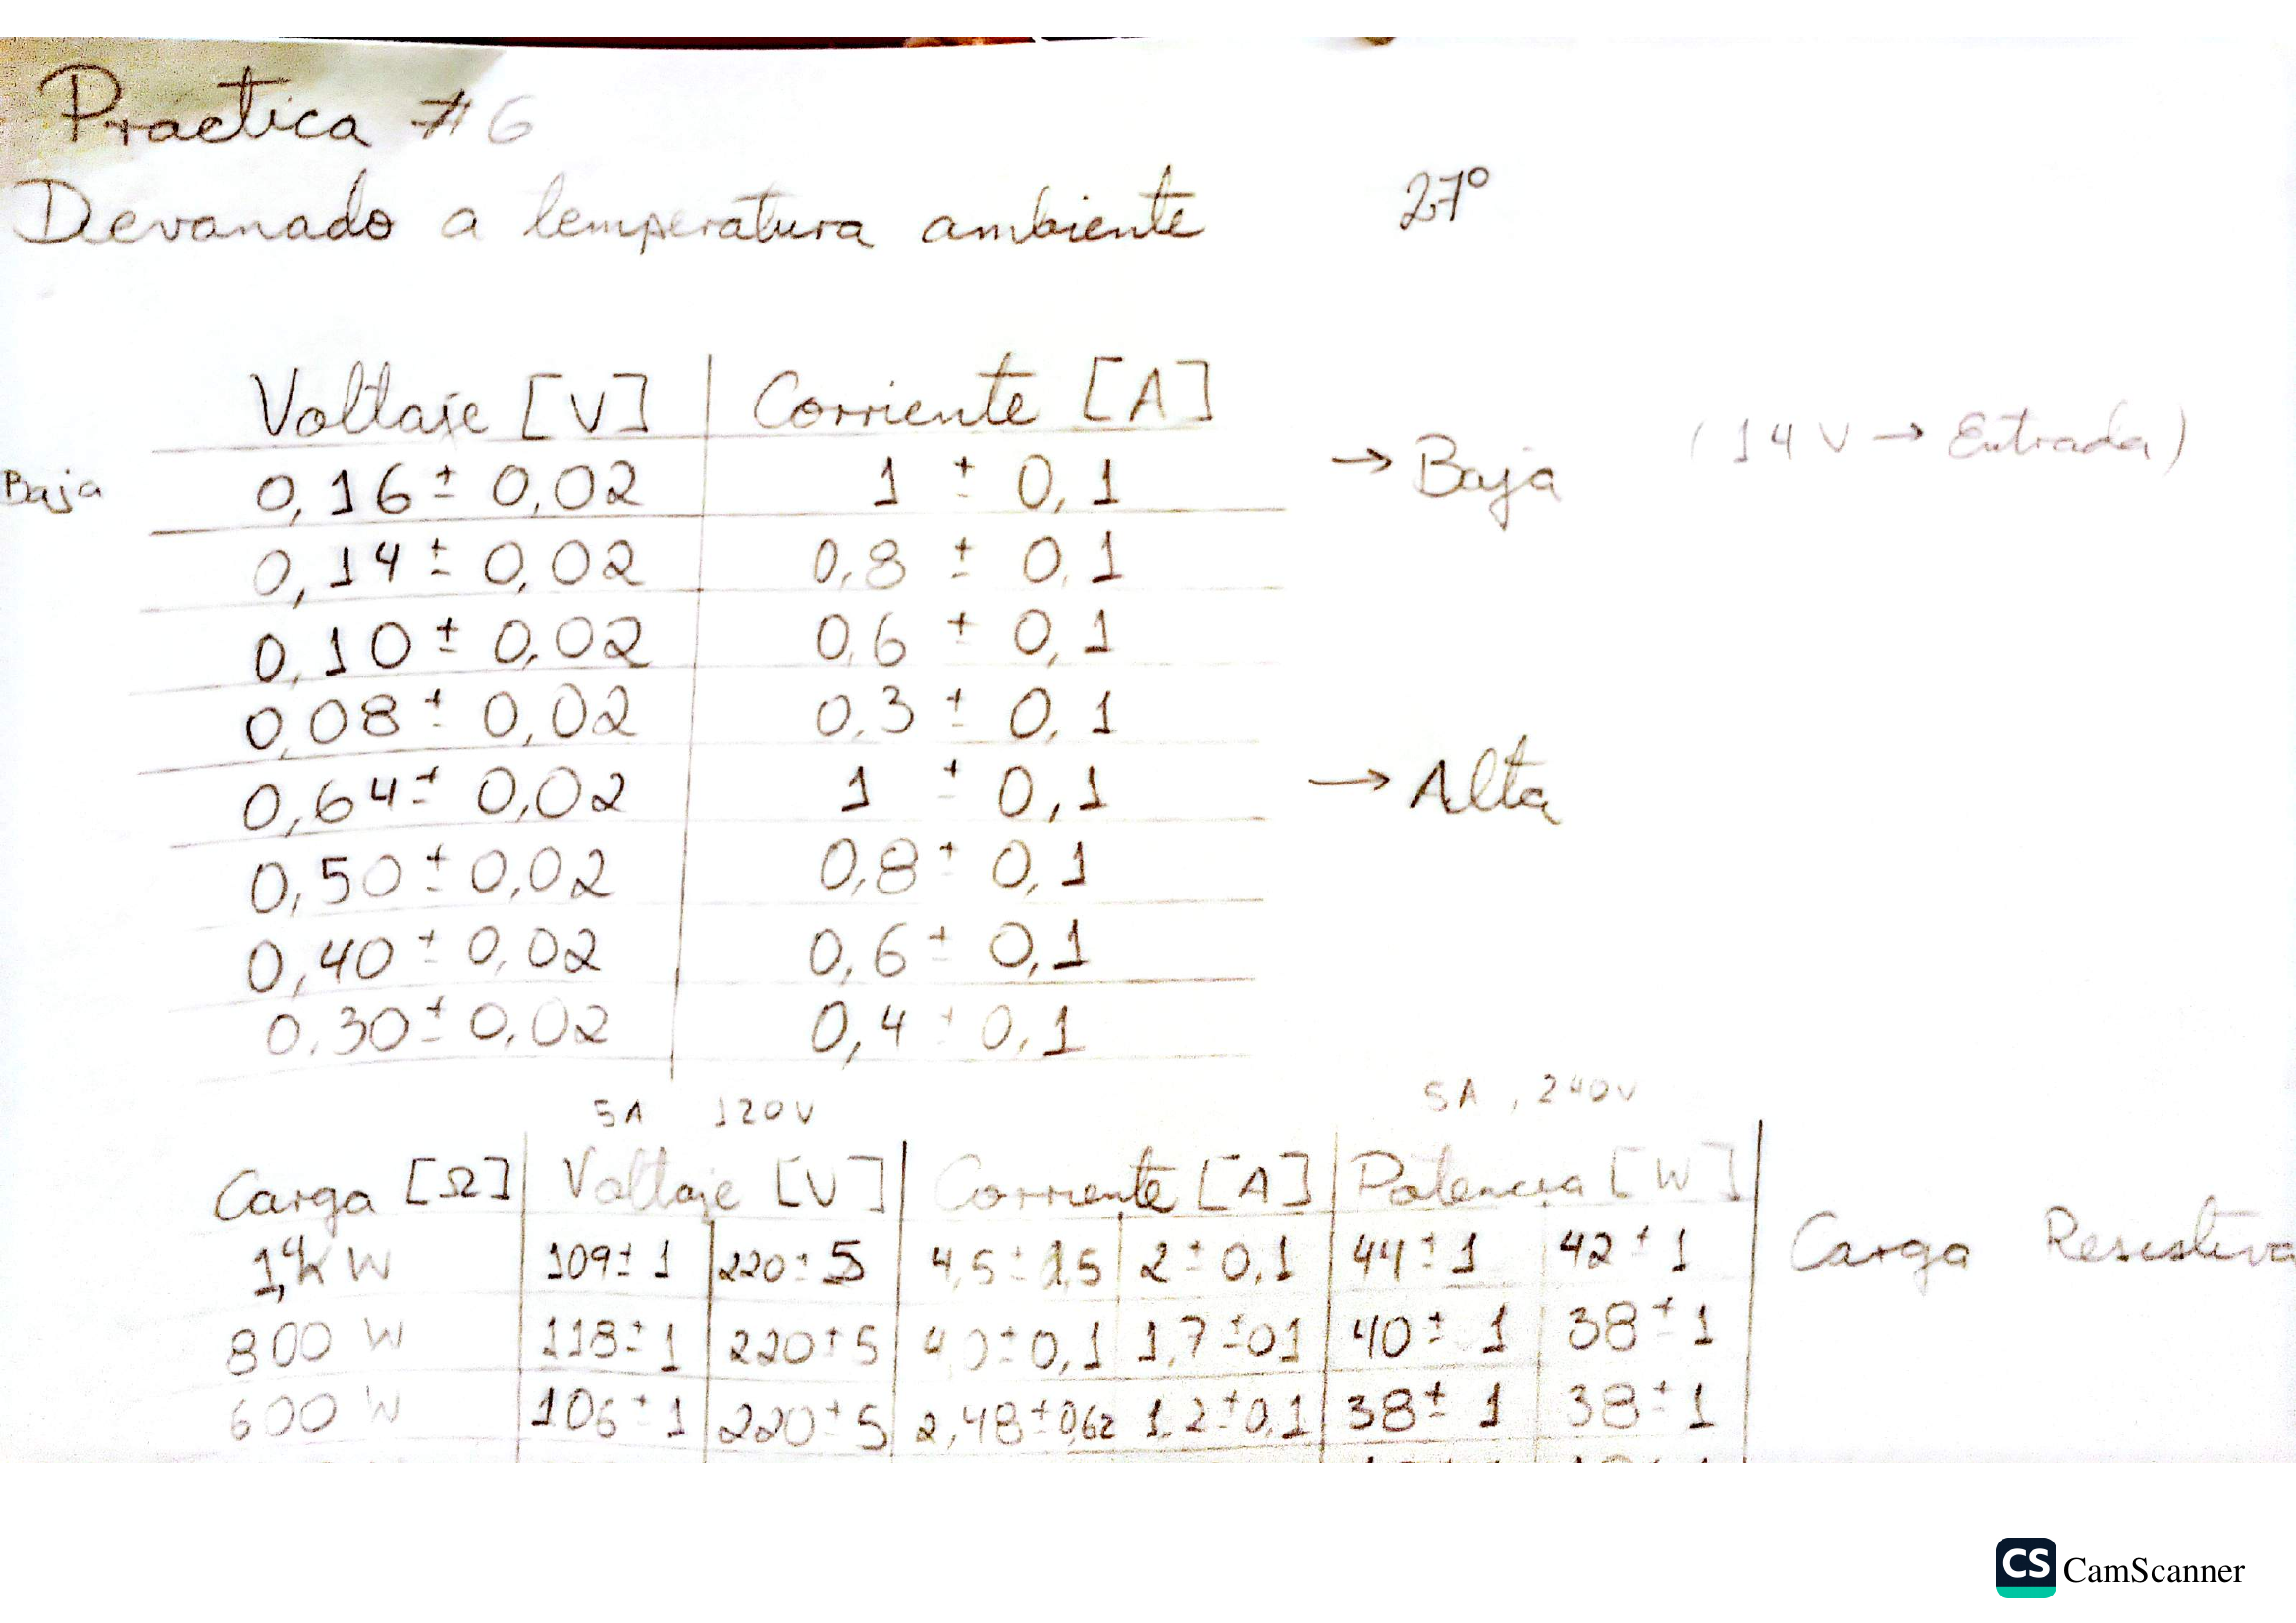
\includegraphics[width=\textwidth]{imagenes/hoja-datos-1.png}
    \caption{Hoja de datos original de laboratorio — Página 1.}
    \label{fig:hoja_datos_1}
\end{figure}

\begin{figure}[H]
    \centering
    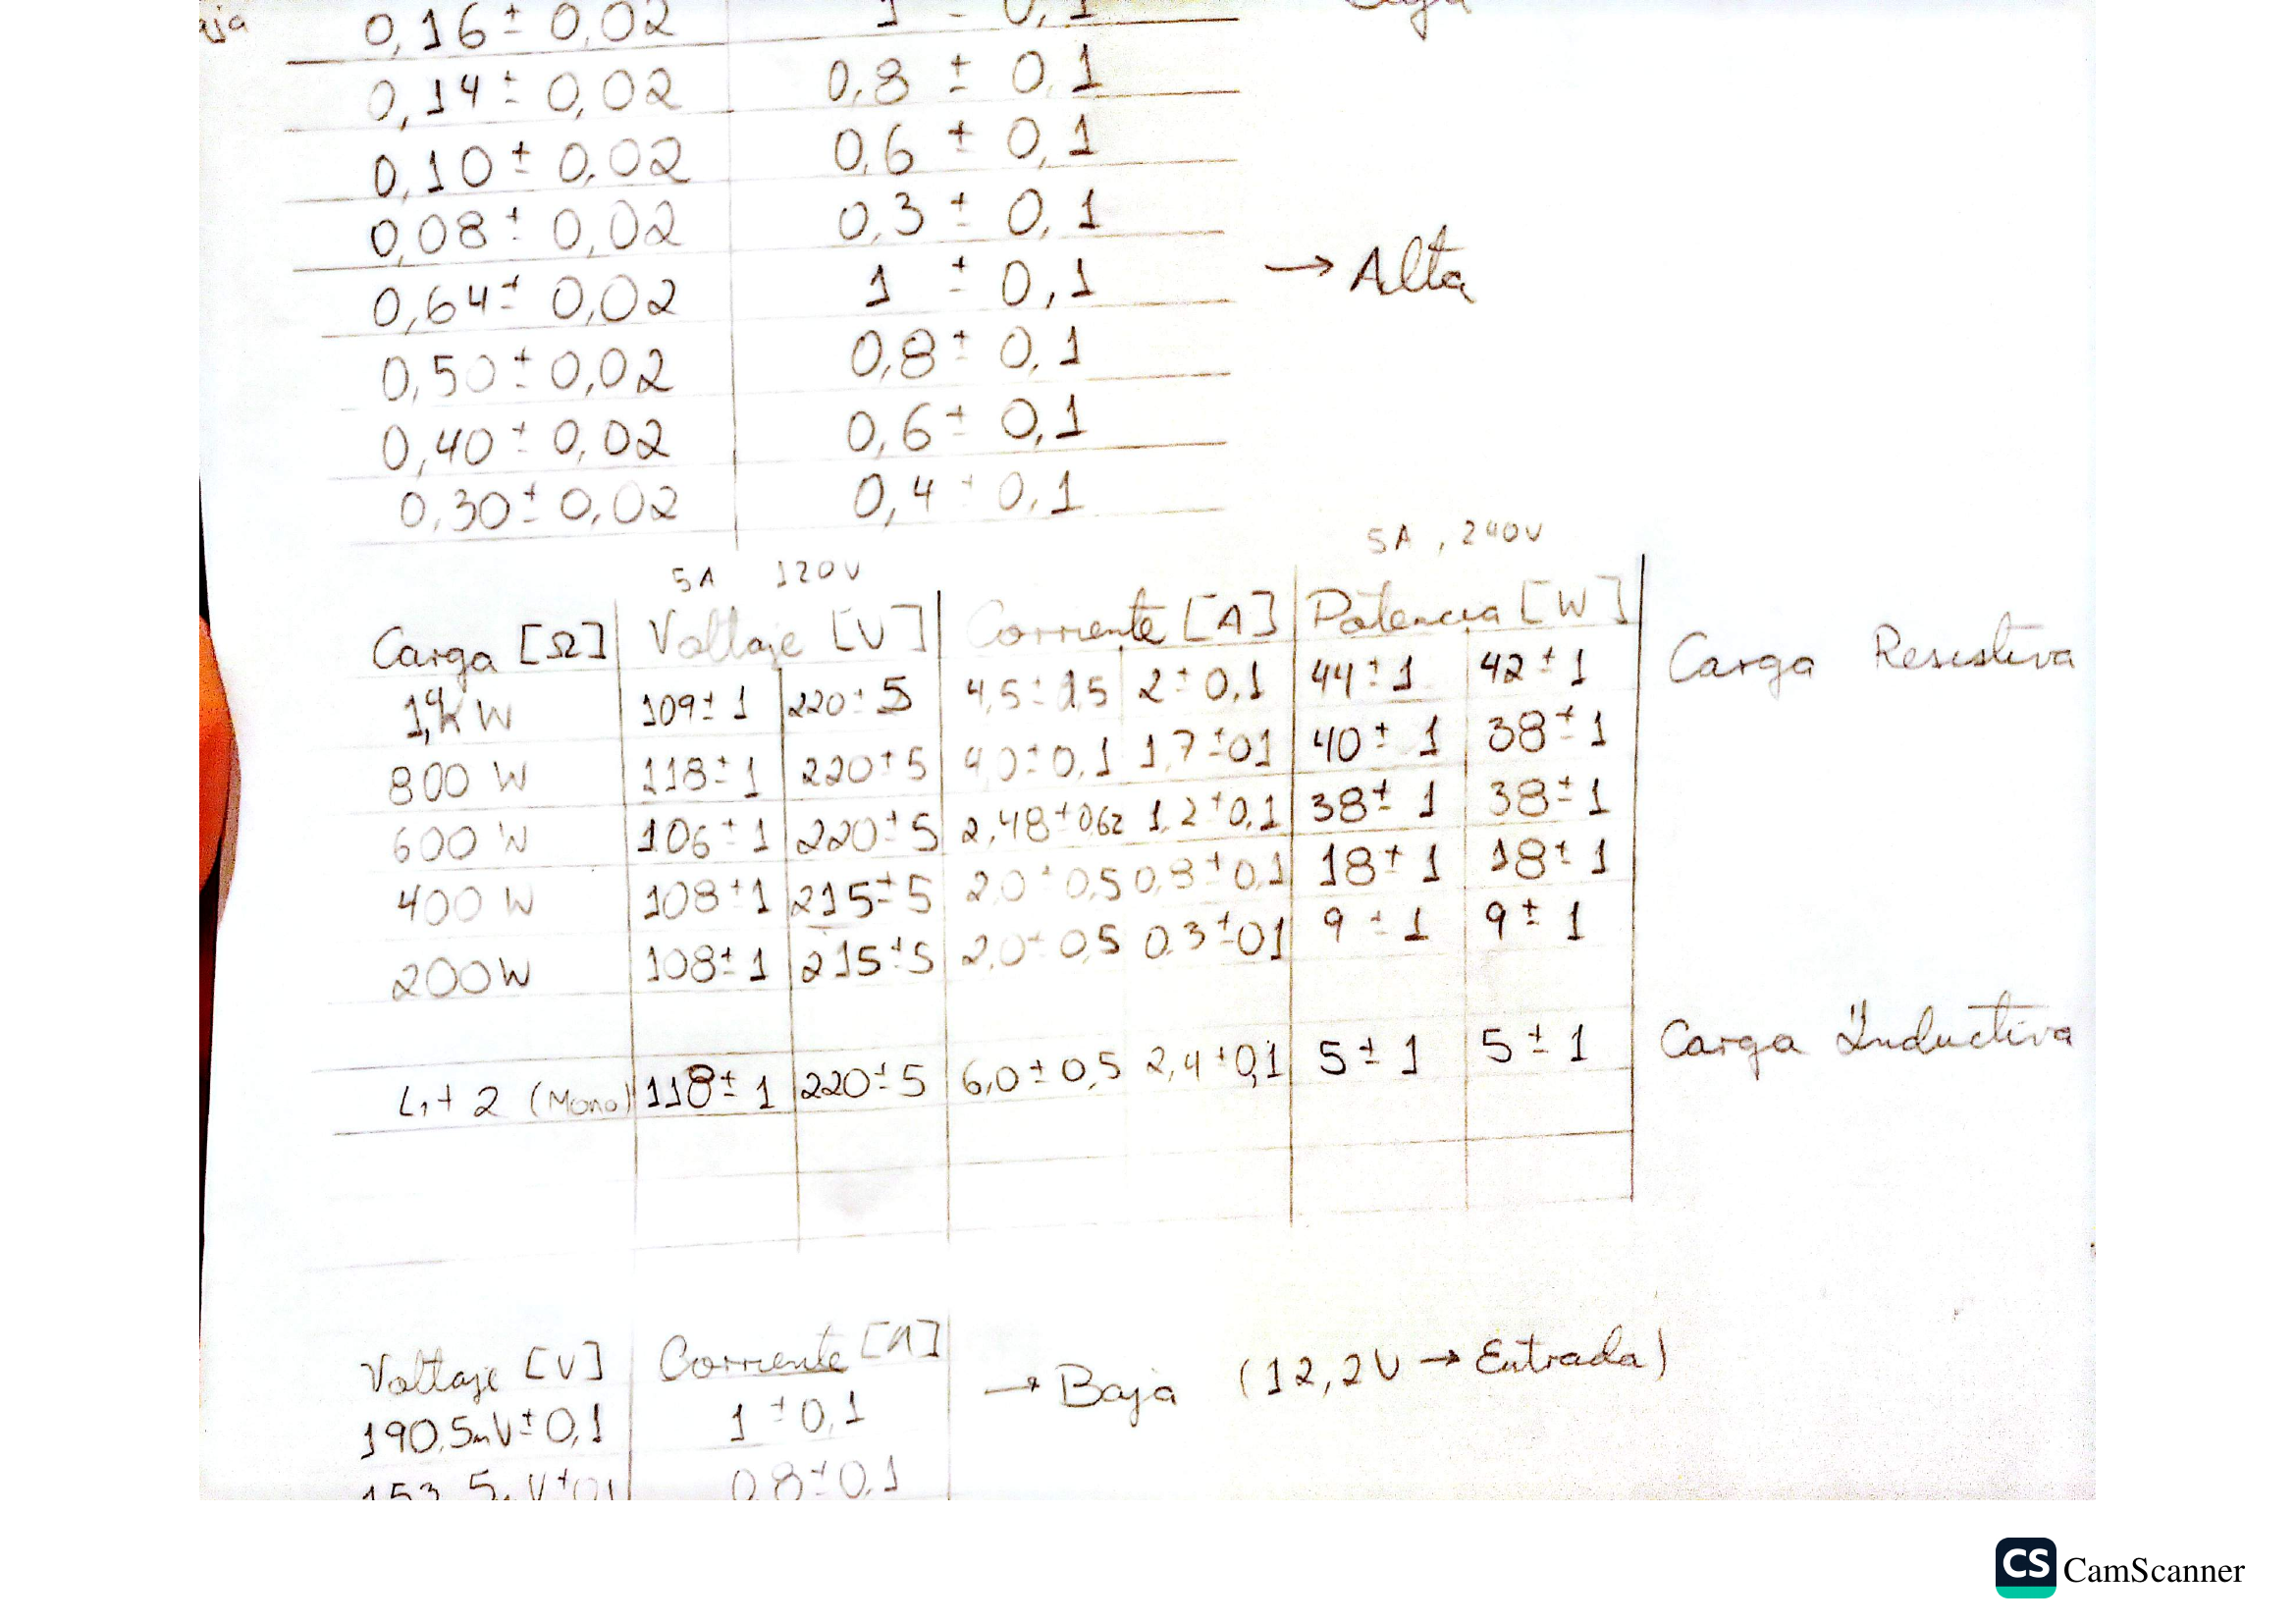
\includegraphics[width=\textwidth]{imagenes/hoja-datos-2.png}
    \caption{Hoja de datos original de laboratorio — Página 2.}
    \label{fig:hoja_datos_2}
\end{figure}

\begin{figure}[H]
    \centering
    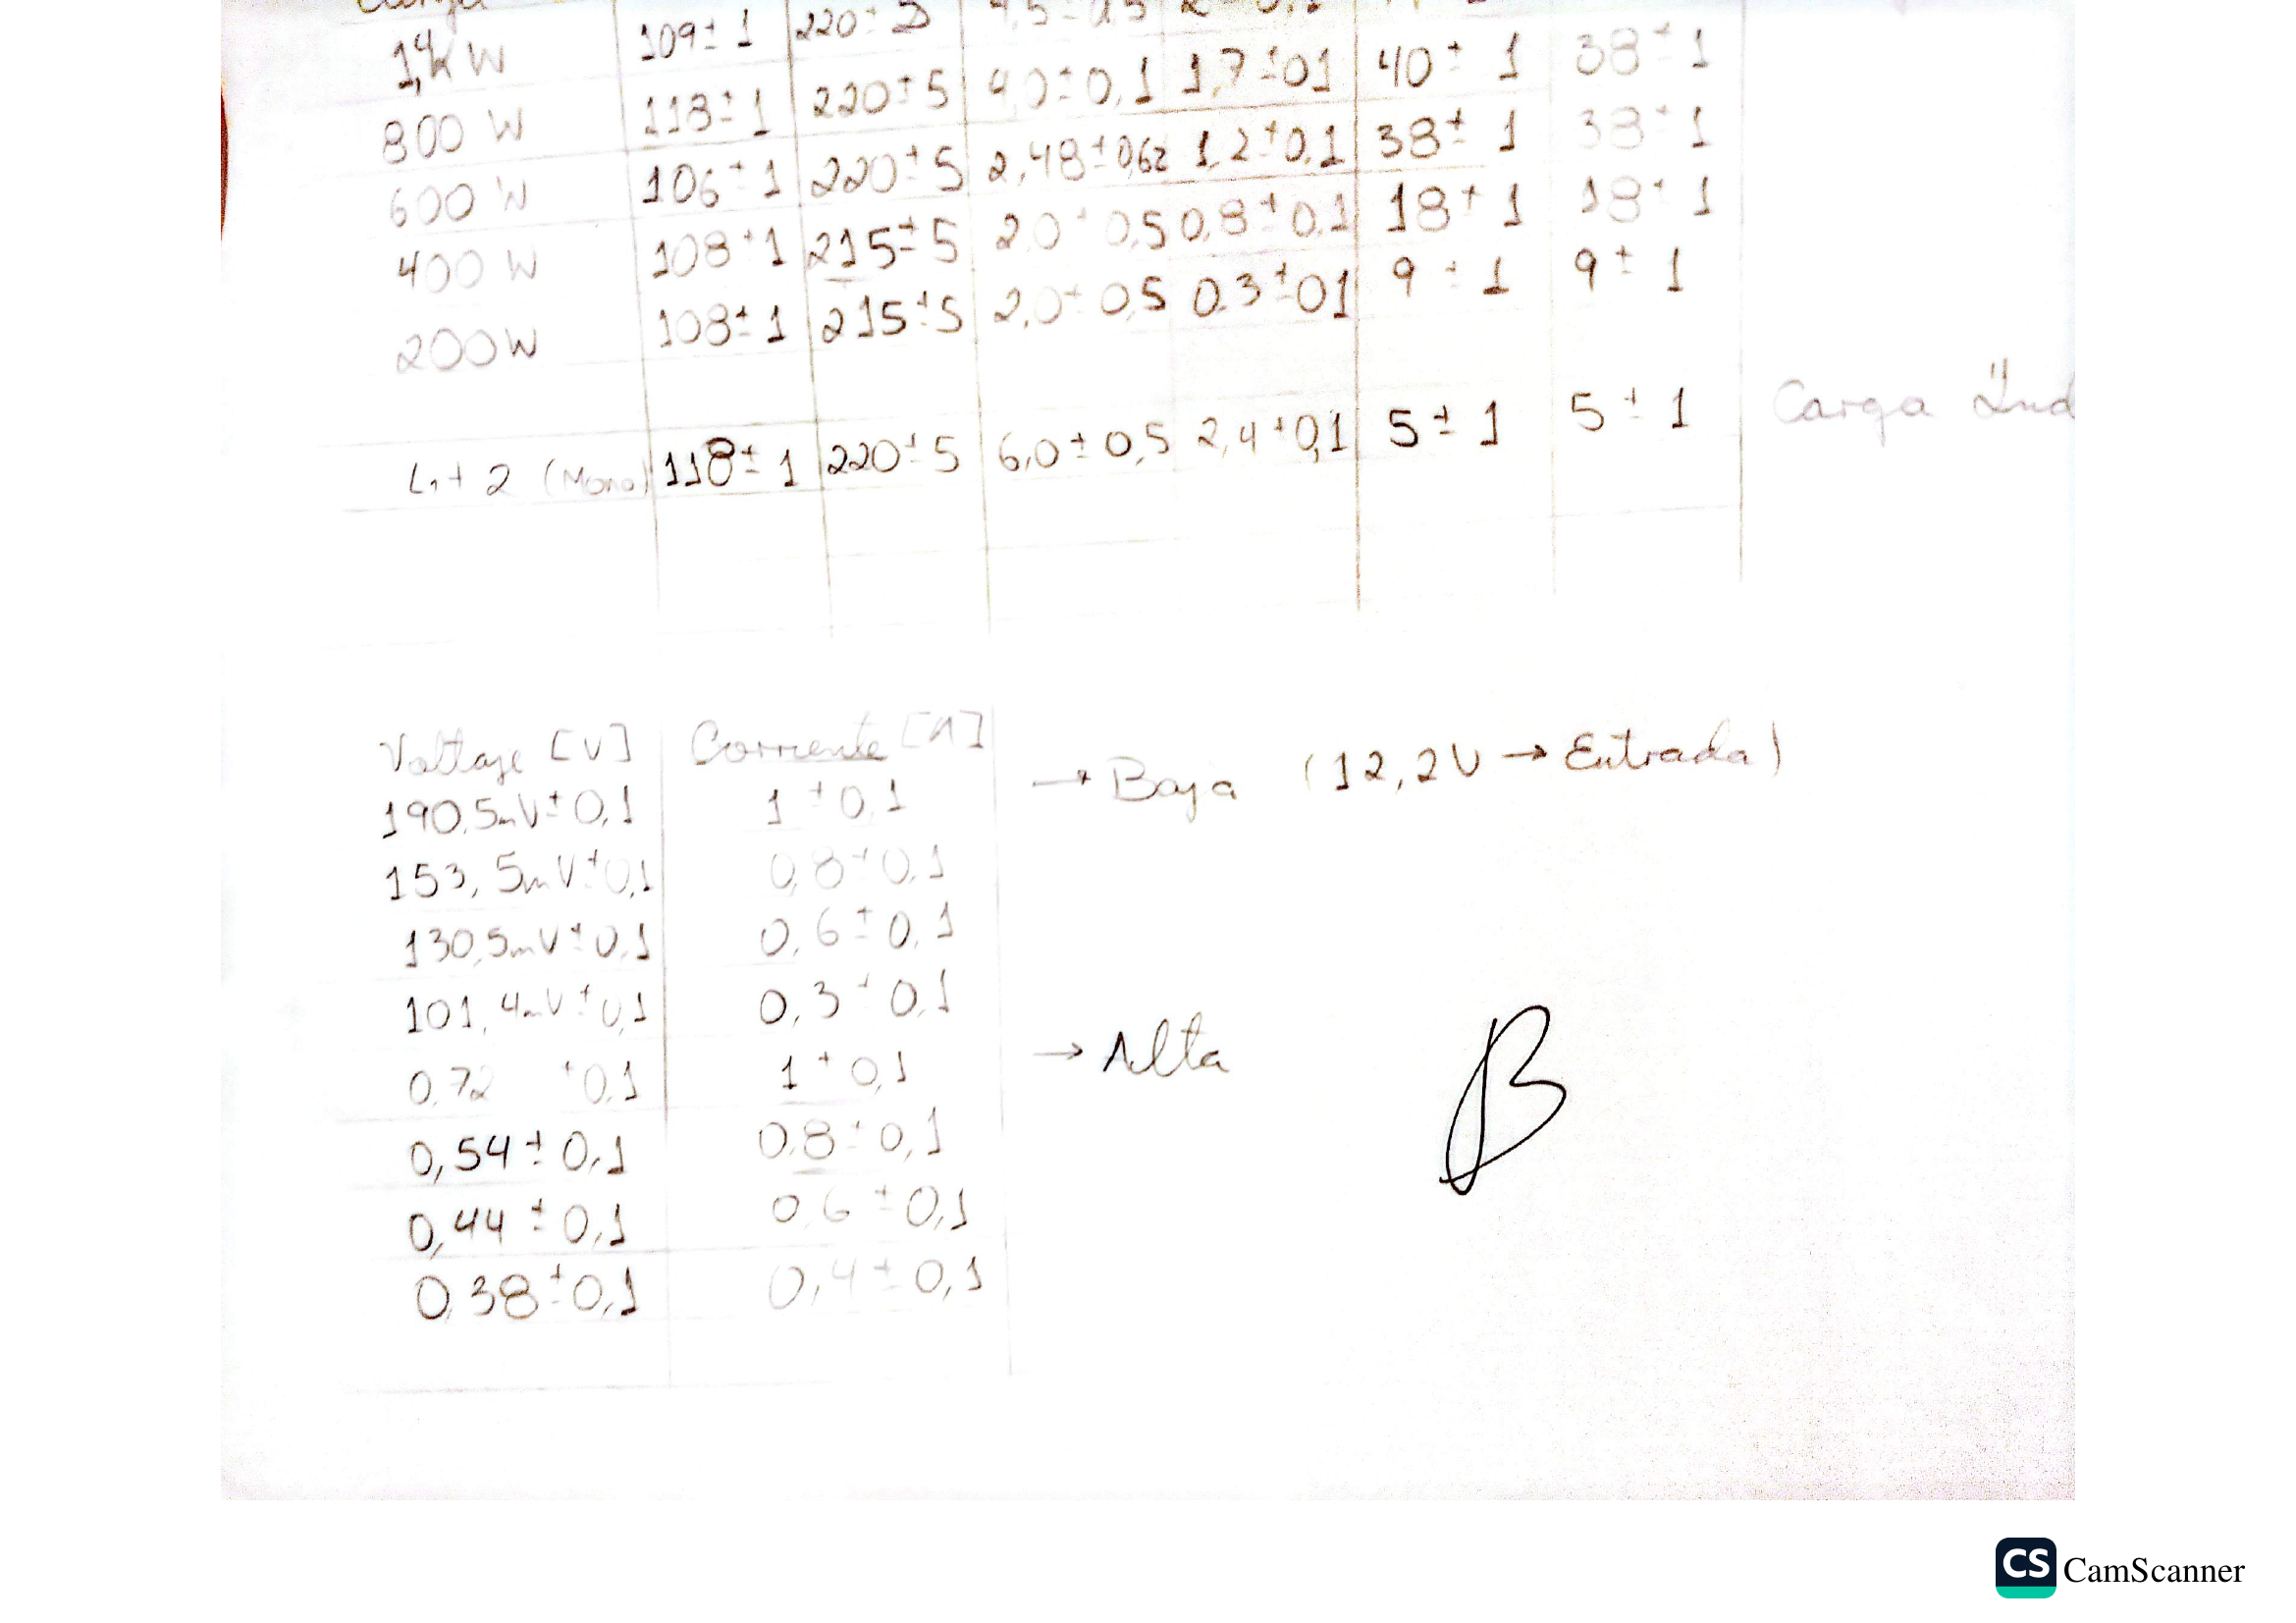
\includegraphics[width=\textwidth]{imagenes/hoja-datos-3.png}
    \caption{Hoja de datos original de laboratorio — Página 3.}
    \label{fig:hoja_datos_3}
\end{figure}

\end{document}
